\chapter{Generative Deep Learning}\label{chp:generative_deep_learning}
\minitoc

\section{Intro to Deep Generative Models}

What is Generative Modeling?

Generative modeling can be broadly defined as follows:
Generative modeling is a branch of machine learning that involves training a model to produce new data that is similar to a given dataset~\cite{foster2022generative}.

Discriminative models vs Generative models

\paragraph{The Generative Modeling Framework}

\begin{itemize}
	\item We have a dataset of Observations $\mathbf{X}$. \item We assume that the observations have been generated according to some unknown distribution \(\mathcal{P}_{\textrm{data}}\)
	\item We want to build a generative model \(\mathcal{P}_{\textrm{model}}\) that mimics \(\mathcal{P}_{\textrm{data}}\) to generate observations that appear to have been drawn from \(\mathcal{P}_{\textrm{data}}\)
	\item Therefore, the desirable properties of \(\mathcal{P}_{\textrm{data}}\) are:

	      1. Accuracy: if \(\mathcal{P}_{\textrm{model}}\)  is high for a generated observation, it should look like it has been drawn from \(\mathcal{P}_{\textrm{data}}\). If \(\mathcal{P}_{\textrm{model}}\) is low, it should look like it has not been drawn from \(\mathcal{P}_{\textrm{data}}\)

	      2. Generation: it should be possible  to easily sample a new observation from \(\mathcal{P}_{\textrm{model}}\)

	      3. Representation:  it should be possible to understand how different high-level features in the data are represented by \(\mathcal{P}_{\textrm{model}}\)
\end{itemize}

\paragraph{Generative Model Taxonomy}

\begin{itemize}
	\item Explicitly model the density function, but constrain the model in some way, so that the density function s tractable (i.e. it can be calculated)
	\item Explicitly model a tractable approximation of the density function.
	\item Implicitly model the density function, through a stochastic process that directly generates data.
\end{itemize}


\begin{figure}
	\begin{center}
		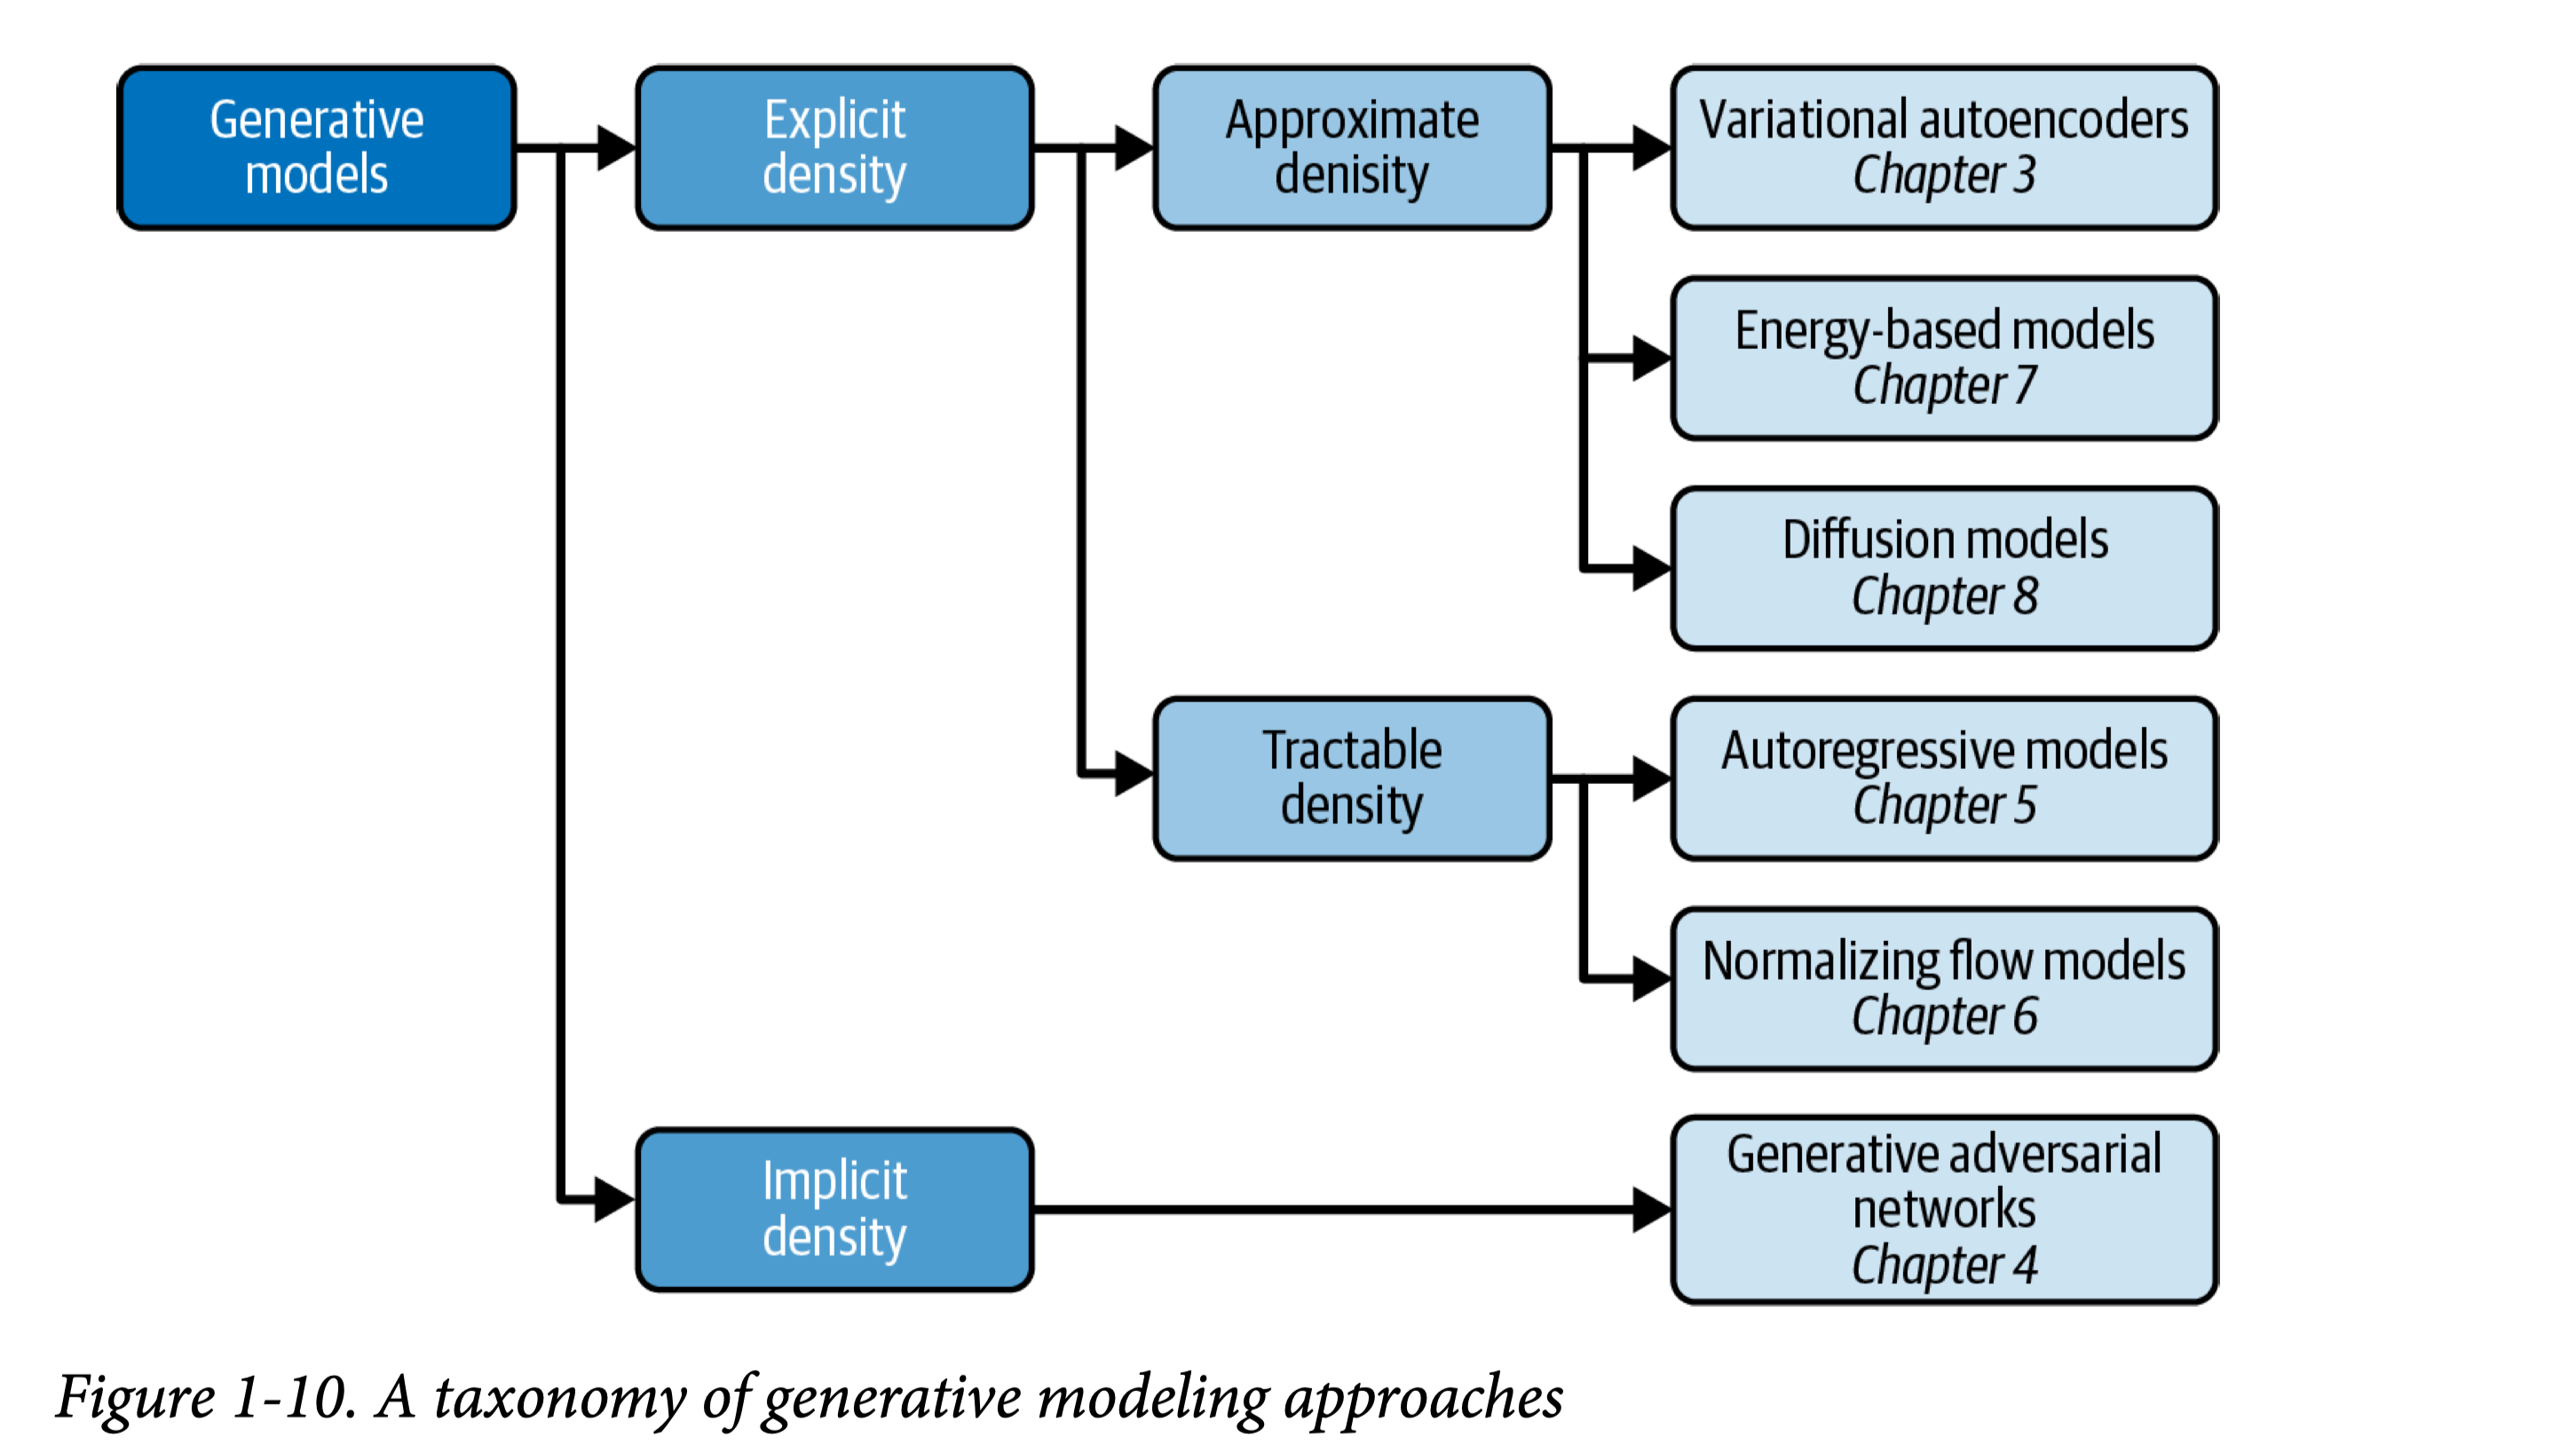
\includegraphics[width=0.95\textwidth]{figures/generative_model_taxonomy}
	\end{center}
	\caption{Generative Models Taxonomy}\label{fig:gmodel_taxonomy}
\end{figure}


If you do choose to use batch normalization before activation, you can remember the order using the acronym \textbf{BAD (batch normalization, activation, then dropout)}

\section{Variational Autoencoders}

\paragraph{The Reparameterization Trick}

Rather than sample directly from a normal distribution with parameters z\_mean and z\_log\_var, we can sample epsilon from a standard normal and then manually adjust the sample to have the correct mean and variance.
This is known as the reparameterization trick, and it’s important as it means gradients can backpropagate freely through the layer.
By keeping all of the randomness of the layer contained within the variable epsilon, the partial derivative of the layer output with respect to its input can be shown to be deterministic (i.e., independent of the random epsilon), which is essential for backpropagation through the layer to be possible.

\paragraph{\gls{kl} Divergence}

\[
	D_{\mathrm{KL}}\left[N\left(\mu,\sigma\right)||N\left(0,1\right)\right] = \frac{1}{2} \sum_{i=1}^n \left(\sigma_i^2 + \mu_i^2 - 1 - \log \sigma_i^2\right)
	.\]


In summary, the \gls{kl}  divergence term penalizes the network for encoding observations to  z\_mean and  z\_log\_var  variables that differ significantly from the parameters of a standard normal distribution, namely \( z\_mean = 0 \) and \( z\_log\_var = 0 \).

Why does this addition to the loss function help?

Firstly, we now have a well-defined distribution that we can use for choosing points in the latent space—the standard normal distribution.
Secondly, since this term tries to force all encoded distributions toward the standard normal distribution, there is less chance that large gaps will form between point clusters.
Instead, the encoder will try to use the space around the origin symmetrically and efficiently.

In the original \gls{vae}  paper, the loss function for a VAE was simply the addition of the reconstruction loss and the KL divergence loss term.
A variant on this (the $\beta$-VAE) includes a factor that weights the \gls{kl}  divergence to ensure that it is well balanced with the reconstruction loss.
If we weight the reconstruction loss too heavily, the \gls{kl} loss will not have the desired regulatory effect and we will see the same problems that we experienced with the plain autoencoder.
If the \gls{kl}  divergence term is weighted too heavily, the \gls{kl}  divergence loss will dominate and the reconstructed images will be poor. This weighting term is one of the parameters to tune when you’re training your VAE~\cite{foster2022generative}.

\paragraph{Latent Space Arithmetic}

One benefit of mapping images into a lower-dimensional latent space is that we can perform arithmetic on vectors in this latent space that has a visual analogue when decoded back into the original image domain~\pautoref{fig:vae_latent_space_arithmetic}.

For example, suppose we want to take an image of somebody who looks sad and give them a smile.
To do this we first need to find a vector in the latent space that points in the direction of increasing smile.
Adding this vector to the encoding of the original image in the latent space will give us a new point which, when decoded, should give us a more smiley version of the original image~\cite{foster2022generative}.

\begin{figure}
	\begin{center}
		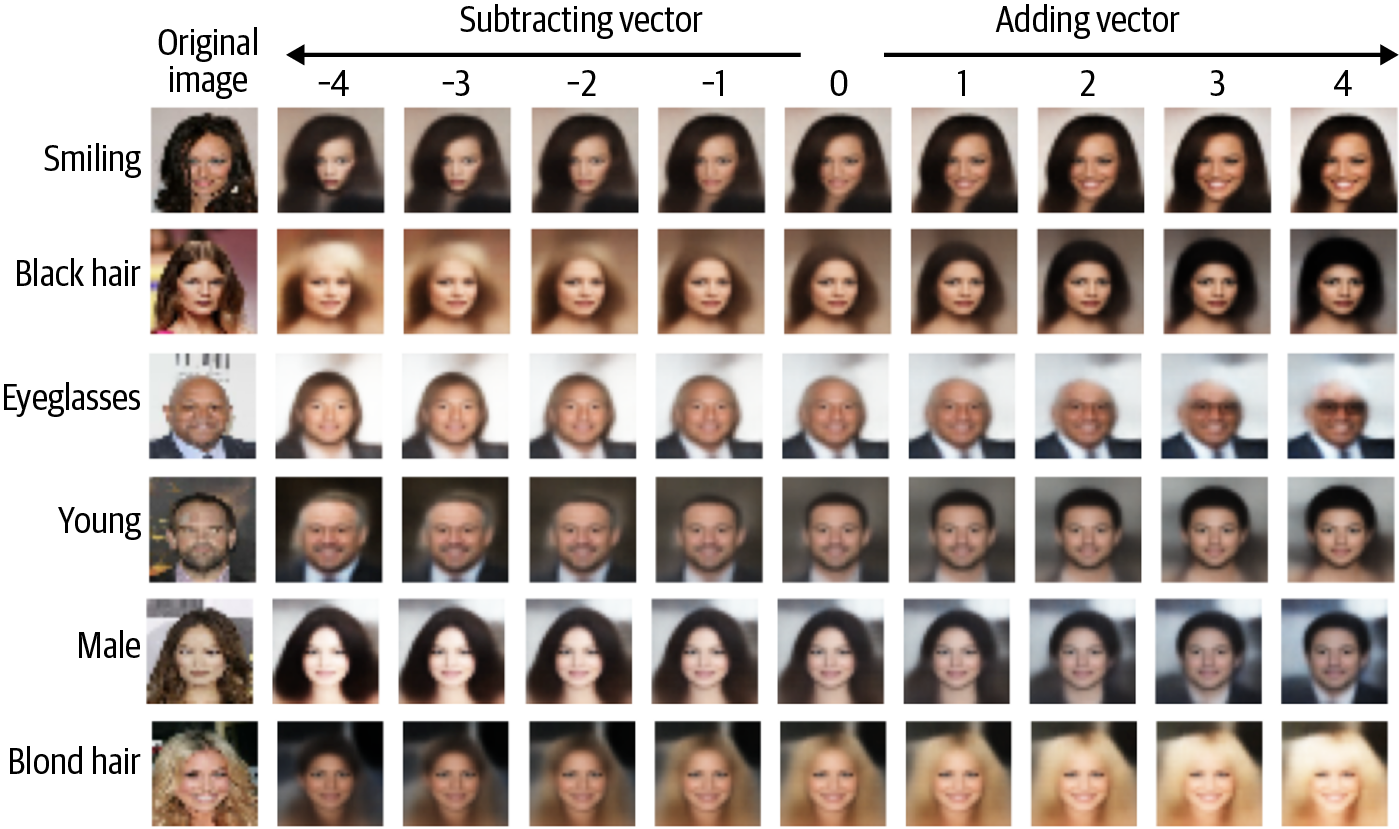
\includegraphics[width=0.95\textwidth]{figures/vae_latent_space_arithmetic}
	\end{center}
	\caption{Adding and subtracting features to and from faces}\label{fig:vae_latent_space_arithmetic}
\end{figure}

\section{Generative Adversarial Networks}

\paragraph{Upsampling vs Transposed Convolution}

The UpSampling2D layer simply repeats each row and column of its input in order to double the size.
The Conv2D layer with stride 1 then performs the convolution operation.
It is a similar idea to convolutional transpose, but instead of filling the gaps between pixels with zeros, upsampling just repeats the existing pixel values.

It has been shown that the Conv2DTranspose method can lead to artifacts, or small checkerboard patterns in the output image (see~\autoref{fig:upsampling}) that spoil the quality of the output.
However, they are still used in many of the most impressive \glspl{gan}  in the literature and have proven to be a powerful tool in the deep learning practitioner’s toolbox.

\begin{figure}
	\begin{center}
		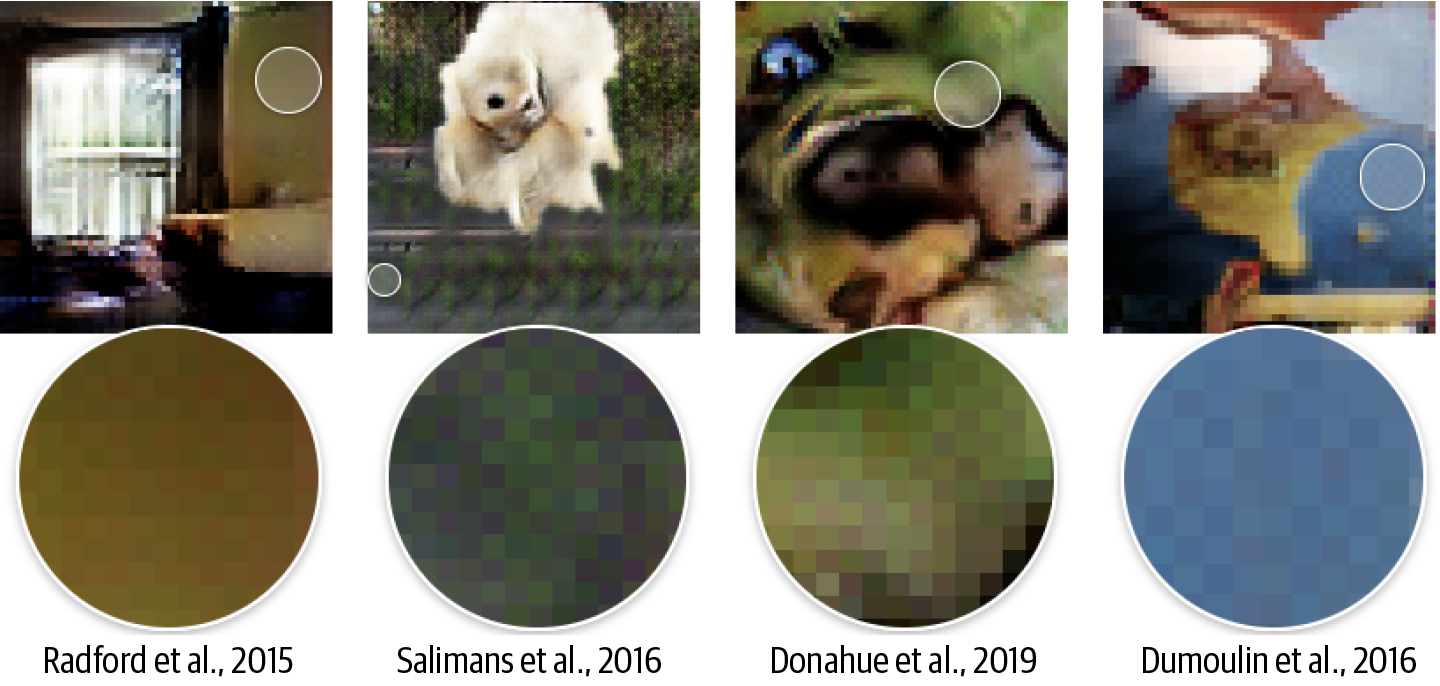
\includegraphics[width=0.9\textwidth]{figures/upsampling}
	\end{center}
	\caption{Artifacts when using convolutional transpose layers}\label{fig:upsampling}
\end{figure}

\paragraph{Adding Noise to the Labels}

A useful trick when training \glspl{gan}  is to add a small amount of random noise to the training labels.
This helps to improve the stability of the training process and sharpen the generated images.
This label smoothing acts as way to tame the discriminator, so that it is presented with a more challenging task and doesn’t overpower the generator.

Another requirement of a successful generative model is that it doesn’t only reproduce images from the training set.
To test this, we can find the image from the training set that is closest to a particular generated example. A good measure for distance is the L1 distance, defined as:

\[
	\mathrm{L1}(\mathbf{a},\mathbf{b}) = \frac{1}{n} \sum_{i=1}^n |a_i - b_i|
	.\]

\subsection{\gls{gan} Training Tips}

While \glspl{gan}  are a major breakthrough for generative modeling, they are also notoriously difficult to train.
We will explore some of the most common problems and challenges encountered when training \glspl{gan}  in this section, alongside potential solutions.
In the next section, we will look at some more fundamental adjustments to the \gls{gan} framework that we can make to remedy many of these problems~\cite{foster2022generative}.

\paragraph{Discriminator overpowering the generator}

If the discriminator becomes too strong, the signal from the loss function becomes too weak to drive any meaningful improvements in the generator.
In the worst-case scenario, the discriminator perfectly learns to separate real images from fake images and the gradients vanish completely, leading to no training whatsoever,

If you find your discriminator loss function collapsing, you need to find ways to weaken the discriminator. Try the following suggestions:

\begin{itemize}
	\item Increase the rate parameter of the Dropout layers in the discriminator to dampen the amount of information that flows through the network.
	\item Reduce the learning rate of the discriminator.
	\item Reduce the number of convolutional filters in the discriminator.
	\item Add noise to the labels when training the discriminator.
	\item Flip the labels of some images at random when training the discriminator.
\end{itemize}

\paragraph{Generator overpowering the discriminator}

If the discriminator is not powerful enough, the generator will find ways to easily trick the discriminator with a small sample of nearly identical images.
This is known as mode collapse.

For example, suppose we were to train the generator over several batches without updating the discriminator in between.
The generator would be inclined to find a single observation (also known as a mode) that always fools the discriminator and would start to map every point in the latent input space to this image.
Moreover, the gradients of the loss function would collapse to near 0, so it wouldn’t be able to recover from this state.

Even if we then tried to retrain the discriminator to stop it being fooled by this one point, the generator would simply find another mode that fools the discriminator, since it has already become numb to its input and therefore has no incentive to diversify its output.

If you find that your generator is suffering from mode collapse, you can try strengthening the discriminator using the opposite suggestions to those listed in the previous section.
Also, you can try reducing the learning rate of both networks and increasing the batch size.

\paragraph{Uninformative Loss}

Since the deep learning model is compiled to minimize the loss function, it would be natural to think that the smaller the loss function of the generator, the better the quality of the images produced.
However, since the generator is only graded against the current discriminator and the discriminator is constantly improving, we cannot compare the loss function evaluated at different points in the training process.
Indeed the loss function of the generator actually increases over time, even though the quality of the images is clearly improving.
This lack of correlation between the generator loss and image quality sometimes makes \gls{gan} training difficult to monitor.

\paragraph{Hyperparameter}

As we have seen, even with simple GANs, there are a large number of hyperparameters to tune.
As well as the overall architecture of both the discriminator and the generator, there are the parameters that govern batch normalization, dropout, learning rate, activation layers, convolutional filters, kernel size, striding, batch size, and latent space size to consider.
GANs are highly sensitive to very slight changes in all of these parameters, and finding a set of parameters that works is often a case of educated trial and error, rather than following an established set of guidelines.

\paragraph{\gls{wgangp}}

\gls{wgangp}~\pautoref{fig:wgangp_training} brings a meaningful loss metric that correlates with the generator’s convergence and sample quality, and improved stability of the optimization process.

\begin{figure}
	\begin{center}
		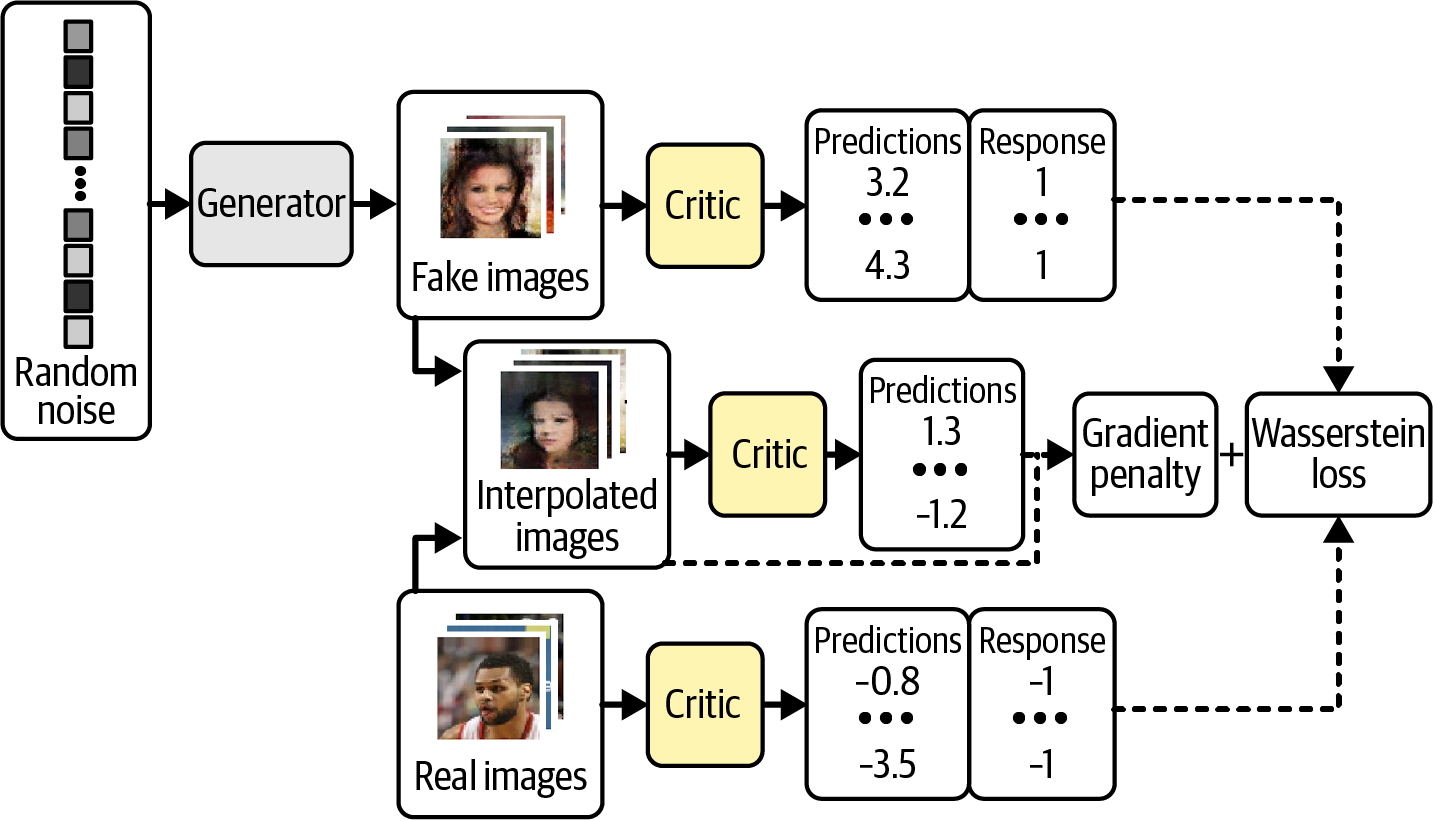
\includegraphics[width=0.95\textwidth]{figures/wgangp_train}
	\end{center}
	\caption{The \gls{wgangp}  critic training process}\label{fig:wgangp_training}
\end{figure}

\begin{equation}
	-\frac{1}{n} \sum_{i=1}^{n} \left(y_i \log\left(p_i\right) + \left(1 - y_i\right)\log \left(1-p_i\right)\right)
	\label{eq:binary_cross_entropy_loss}
\end{equation}

One last consideration we should note before training a \gls{wgangp} is that batch normalization shouldn’t be used in the critic.
This is because batch normalization creates correlation between images in the same batch, which makes the gradient penalty loss less effective.
Experiments have shown that \glspl{wgangp}  can still produce excellent results even without batch normalization in the critic.
We have now covered all of the key differences between a standard GAN and a \gls{wgangp}. To recap:

\begin{itemize}
	\item A \gls{wgangp} uses the Wasserstein loss.
	\item The \gls{wgangp}  is trained using labels of 1 for real and –1 for fake.
	\item There is no sigmoid activation in the final layer of the critic.
	\item Include a gradient penalty term in the loss function for the critic.
	\item Train the critic multiple times for each update of the generator.
	\item There are no batch normalization layers in the critic.
\end{itemize}

\paragraph{\gls{cgan}}

\begin{figure}
	\begin{center}
		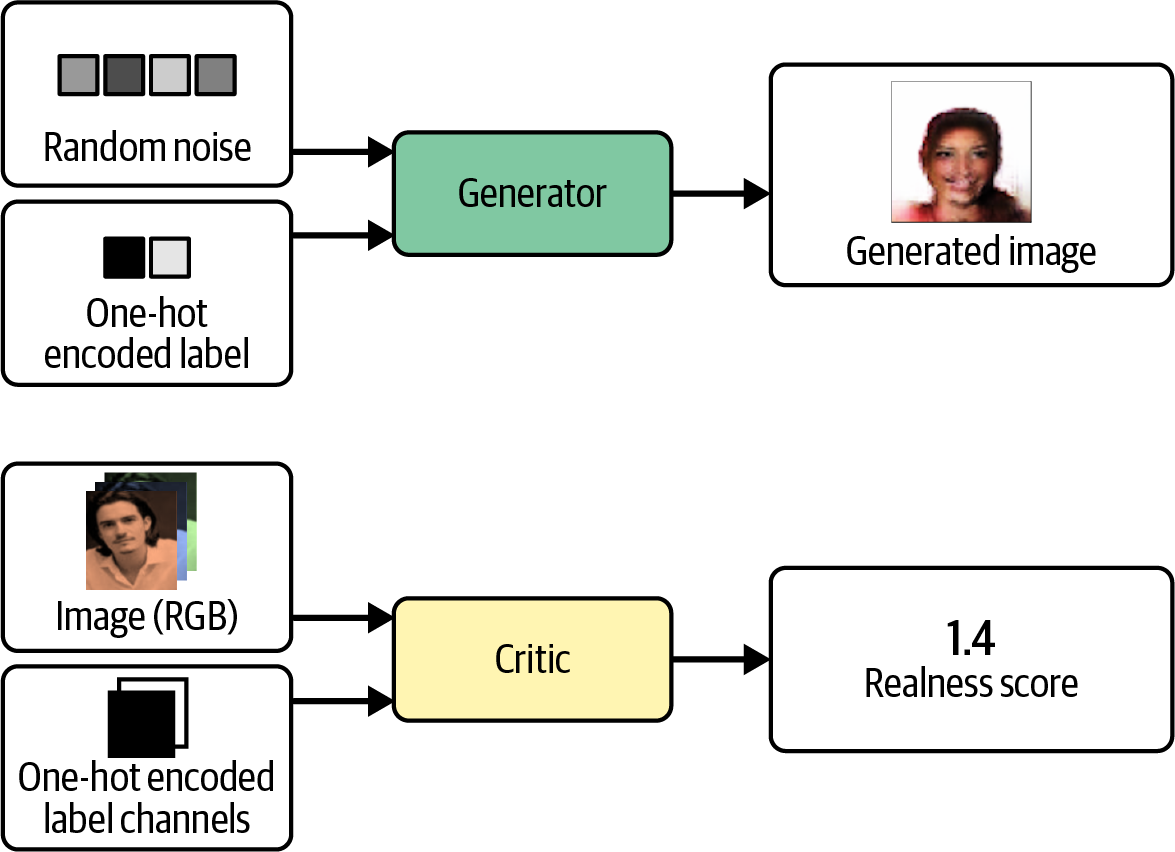
\includegraphics[width=0.95\textwidth]{figures/cgan}
	\end{center}
	\caption{Inputs and outputs of the generator and critic in a CGAN}\label{fig:cgan}
\end{figure}

\paragraph{Summary}

we explored three different \gls{gan} models: the \gls{dcgan}, the more sophisticated \gls{wgangp}, and the \gls{cgan}.

All \glspl{gan} are characterized by a generator versus discriminator (or critic) architecture, with the discriminator trying to ``spot the difference'' between real and fake images and the generator aiming to fool the discriminator.
By balancing how these two adversaries are trained, the \gls{gan} generator can gradually learn how to produce similar observations to those in the training set.

We first saw how to train a \gls{dcgan} to generate images of toy bricks.
It was able to learn how to realistically represent 3D objects as images, including accurate representations of shadow, shape, and texture.
We also explored the different ways in which \gls{gan} training can fail, including mode collapse and vanishing gradients~\cite{foster2022generative}.

\section{Autoregressive Models}

\paragraph{Working with Text Data}

There are several key differences between text and image data that mean that many of the methods that work well for image data are not so readily applicable to text data.
In particular:

\begin{itemize}
	\item Text data is composed of discrete chunks (either characters or words), whereas pixels in an image are points in a continuous color spectrum.
	      We can easily make a green pixel more blue, but it is not obvious how we should go about making the word cat more like the word dog, for example.
	      This means we can easily apply backpropagation to image data, as we can calculate the gradient of our loss function with respect to individual pixels to establish the direction in which pixel colors should be changed to minimize the loss.
	      With discrete text data, we can’t obviously apply backpropagation in the same way, so we need to find a way around this problem.

	\item Text data has a time dimension but no spatial dimension, whereas image data has two spatial dimensions but no time dimension.
	      The order of words is highly important in text data and words wouldn’t make sense in reverse, whereas images can usually be flipped without affecting the content.
	      Furthermore, there are often long-term sequential dependencies between words that need to be captured by the model: for example, the answer to a question or carrying forward the context of a pronoun.
	      With image data, all pixels can be processed simultaneously.

	\item Text data is highly sensitive to small changes in the individual units (words or characters).
	      Image data is generally less sensitive to changes in individual pixel units—a picture of a house would still be recognizable as a house even if some pixels were altered—but with text data, changing even a few words can drastically alter the meaning of the passage, or make it nonsensical.
	      This makes it very difficult to train a model to generate coherent text, as every word is vital to the overall meaning of the passage.

	\item Text data has a rules-based grammatical structure, whereas image data doesn’t follow set rules about how the pixel values should be assigned.
	      For example, it wouldn’t make grammatical sense in any context to write ``The cat sat on the having.''
	      There are also semantic rules that are extremely difficult to model; it wouldn’t make sense to say ``I am in the beach,'' even though grammatically, there is nothing wrong with this statement.
\end{itemize}

\paragraph{Tokenization}

If you use word tokens:

\begin{itemize}
	\item  All text can be converted to lowercase, to ensure capitalized words at the start of sentences are tokenized the same way as the same words appearing in the middle of a sentence.
	      In some cases, however, this may not be desirable; for example, some proper nouns, such as names or places, may benefit from remaining capitalized so that they are tokenized independently.

	\item  The text vocabulary (the set of distinct words in the training set) may be very large, with some words appearing very sparsely or perhaps only once.
	      It may be wise to replace sparse words with a token for unknown word, rather than including them as separate tokens, to reduce the number of weights the neural network needs to learn.

	\item  Words can be stemmed, meaning that they are reduced to their simplest form, so that different tenses of a verb remained tokenized together.
	      For example, browse, browsing, browses, and browsed would all be stemmed to brows.

	\item  You will need to either tokenize the punctuation, or remove it altogether.
	\item  Using word tokenization means that the model will never be able to predict words outside of the training vocabulary.
\end{itemize}

If you use character tokens:

\begin{itemize}
	\item The model may generate sequences of characters that form new words outside of the training vocabulary—this may be desirable in some contexts, but not in others.

	\item Capital letters can either be converted to their lowercase counterparts, or remain as separate tokens.

	\item The vocabulary is usually much smaller when using character tokenization. This is beneficial for model training speed as there are fewer weights to learn in the final output layer.
\end{itemize}

\paragraph{\gls{lstm}}

A recurrent layer has the special property of being able to process sequential input data \(x_{1}, \ldots , x_{n} \).
It consists of a cell that updates its hidden state, \( h_{t}\), as each element of the sequence \( x_{t} \) is passed through it, one timestep at a time.

The hidden state is a vector with length equal to the number of units in the cell.
it can be thought of as the cell’s current understanding of the sequence.
At timestep \( t \), the cell uses the previous value of the hidden state,\( h_{t-1} \), together with the data from the current timestep \( x_{t} \) to produce an updated hidden state vector, \( h_t\).
This recurrent process continues until the end of the sequence.
Once the sequence is finished, the layer outputs the final hidden state of the cell, \( h_n \),
It’s important to remember that all of the cells in this diagram share the same weights (as they are really the same cell).

We represent the recurrent process by drawing a copy of the cell at each timestep and show how the hidden state is constantly being updated as it flows through the cells~\pautoref{fig:recurrent_layer}.

\begin{figure}
	\begin{center}
		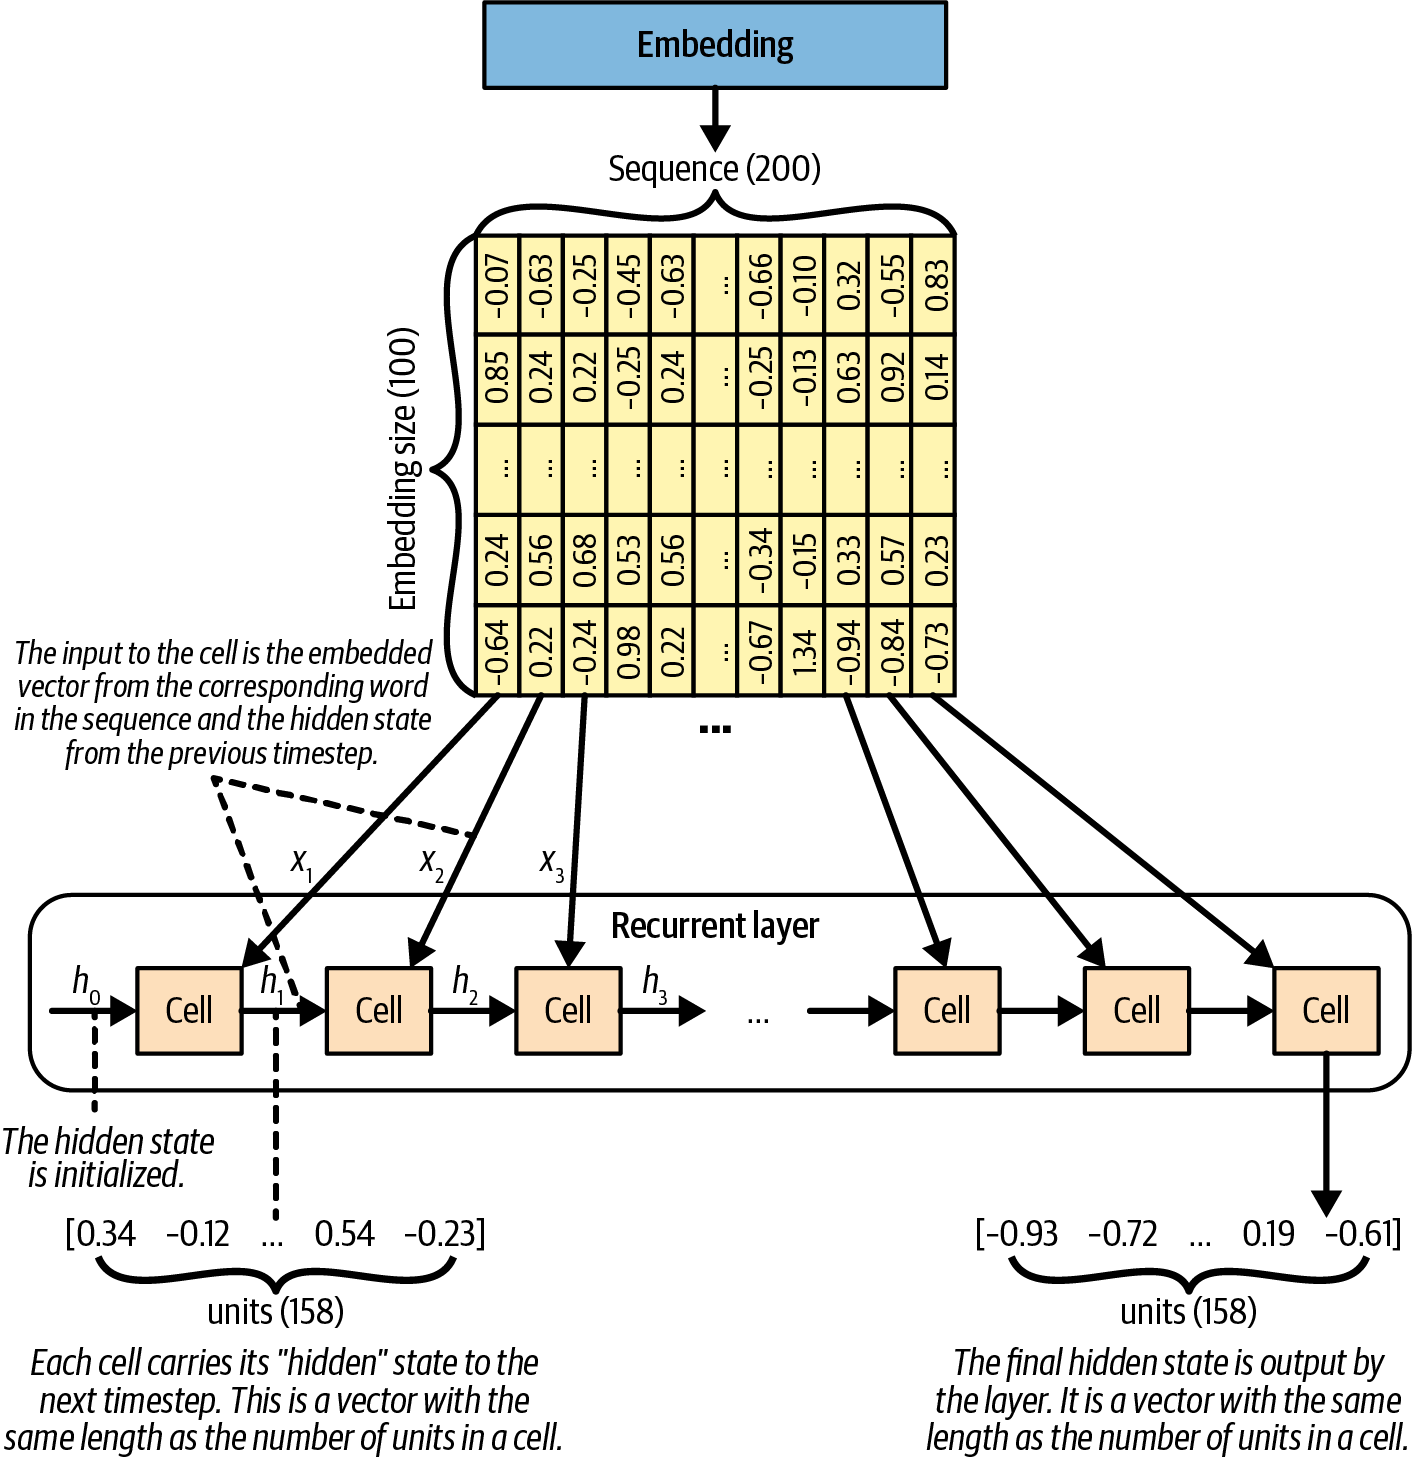
\includegraphics[width=0.95\textwidth]{figures/recurrent_layer}
	\end{center}
	\caption{How a single sequence flows through a recurrent layer}\label{fig:recurrent_layer}
\end{figure}


The hidden state is updated in six steps~\pautoref{fig:lstm_cell}:

\begin{figure}
	\begin{center}
		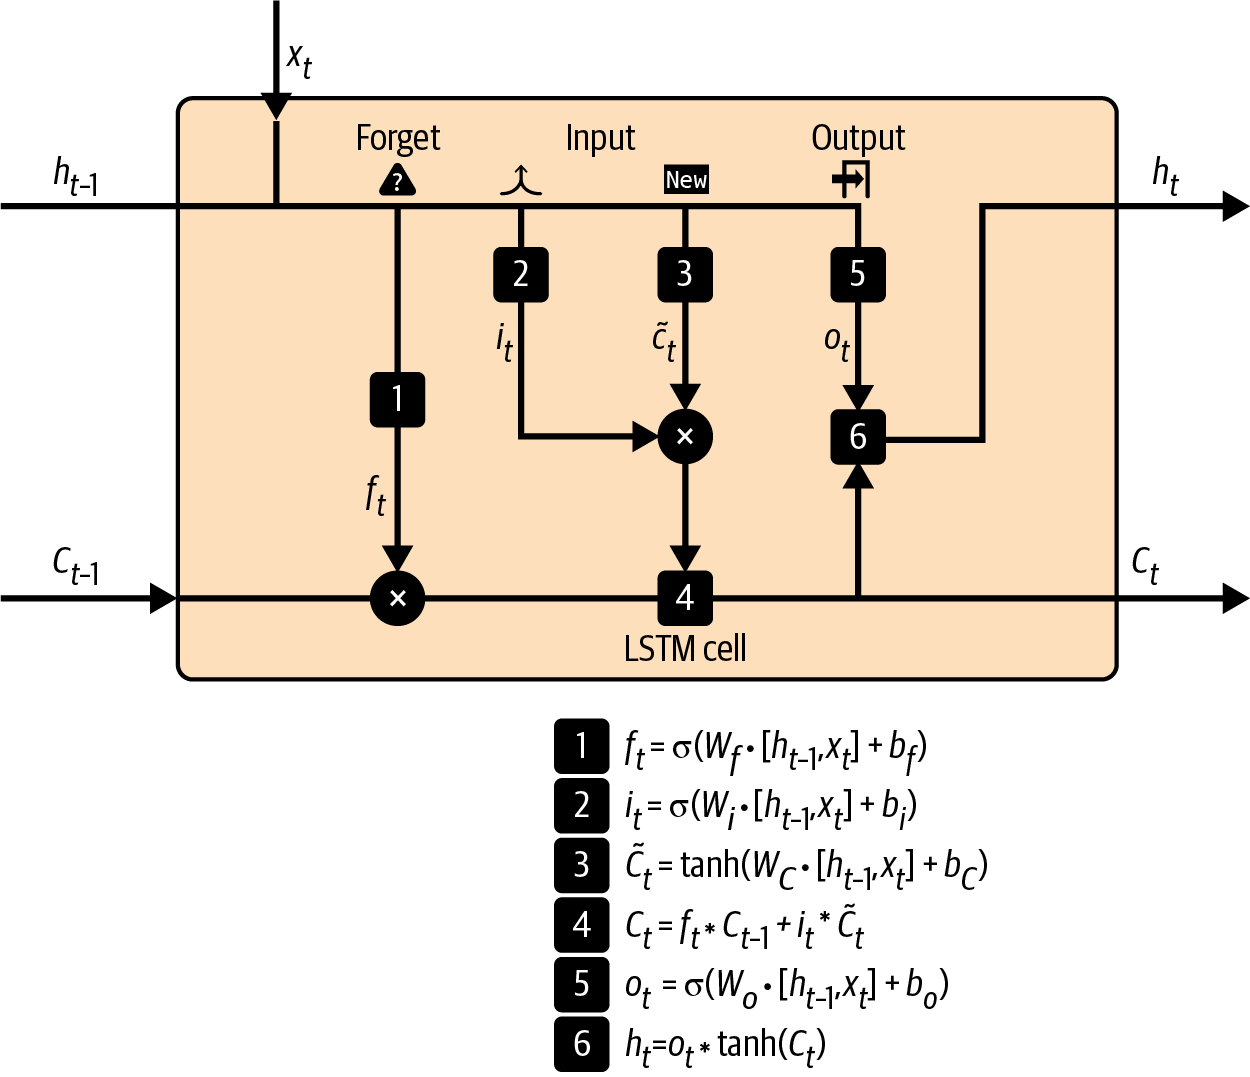
\includegraphics[width=0.95\textwidth]{figures/lstm_cell}
	\end{center}
	\caption{An \gls{lstm} Cell}\label{fig:lstm_cell}
\end{figure}


\begin{enumerate}
	\item The hidden state of the previous timestep, \( h_{t-1} \), and the current word embedding, \( x_t \), are concatenated and passed through the forget gate.
	      This gate is simply a dense layer with weights matrix  \( \mathbf{W}_{f}\) , bias \( b_f \), and a sigmoid activation function.
	      The resulting vector, \( f_tl \), has length equal to the number of units in the cell and contains values between 0 and 1 that determine how much of the previous cell state, \( C_{t-1}\), should be retained.

	\item The concatenated vector is also passed through an input gate that, like the forget gate, is a dense layer with weights matrix \( \mathbf{W}_i\), bias \( b_i \), and a sigmoid activation function.
	      The output from this gate, \( i_t \), has length equal to the number of units in the cell and contains values between 0 and 1 that determine how much new information will be added to the previous cell state, \( C_{t-1}\).

	\item The concatenated vector is passed through a dense layer with weights matrix \( \mathbf{W}_C \), bias \( b_C \), and a tanh activation function to generate a vector \( \tilde{C_t} \) that contains the new information that the cell wants to consider keeping.
	      It also has length equal to the number of units in the cell and contains values between –1 and 1.

	\item \( f_t \) and \( C_{t-1} \) are multiplied element-wise and added to the element-wise multiplication of \( i_t \) and \( \tilde{C_t}\).
	      This represents forgetting parts of the previous cell state and then adding new relevant information to produce the updated cell state, \( C_t \).

	\item The concatenated vector is passed through an output gate: a dense layer with weights matrix \( \mathbf{W}_o \), bias \( b_o \), and a sigmoid activation.
	      The resulting vector, \( o_t \), has length equal to the number of units in the cell and stores values between 0 and 1 that determine how much of the updated cell state, \( C_t \), to output from the cell.

	\item \( o_t\) is multiplied element-wise with the updated cell state, \( C_t \), after a tanh activation has been applied to produce the new hidden state, \( h_t \).
\end{enumerate}

\paragraph{\gls{gru}}

\begin{figure}
	\begin{center}
		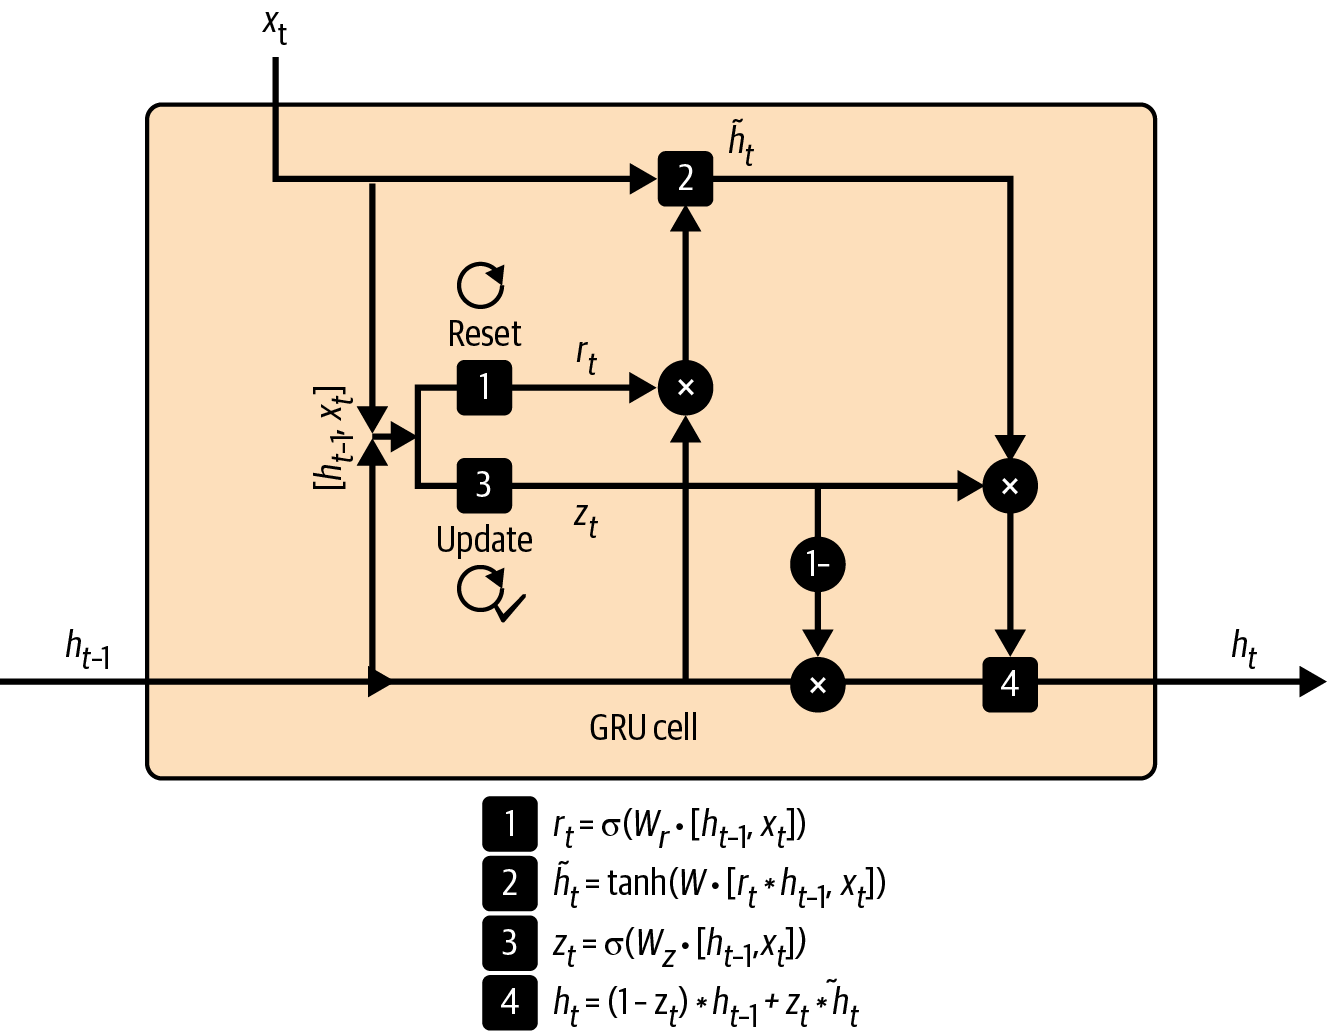
\includegraphics[width=0.95\textwidth]{figures/gru}
	\end{center}
	\caption{A single \gls{gru} cell}\label{fig:gru}
\end{figure}

Another type of commonly used \gls{rnn} layer is the \gls{gru}~\pautoref{fig:gru}.
The key differences from the \gls{lstm} unit are as follows:

\begin{enumerate}
	\item The forget and input gates are replaced by reset and update gates.
	\item There is no cell state or output gate, only a hidden state that is output from the cell.
\end{enumerate}

\section{Normalizing Flow Models}

Normalizing flows share similarities with both autoregressive models and \glspl{vae}.
Like autoregressive models, normalizing flows are able to explicitly and tractably model the data-generating distribution \(\mathcal{P}_{x}\).
Like \glspl{vae}, normalizing flows attempt to map the data into a simpler distribution, such as a Gaussian distribution.
The key difference is that normalizing flows place a constraint on the form of the mapping function, so that it is invertible and can therefore be used to generate new data points.


\paragraph{Summary}

A normalizing flow model is an invertible function defined by a neural network that allows us to directly model the data density via a change of variables.
In the general case, the change of variables equation requires us to calculate a highly complex Jacobian determinant, which is impractical for all but the simplest of examples.

To sidestep this issue, the RealNVP model restricts the form of the neural network, such that it adheres to the two essential criteria: it is invertible and has a Jacobian determinant that is easy to compute.

It does this through stacking coupling layers, which produce scale and translation factors at each step.
Importantly, the coupling layer masks the data as it flows through the network, in a way that ensures that the Jacobian is lower triangular and therefore has a simple-to-compute determinant.
Full visibility of the input data is achieved through flipping the masks at each layer.

By design, the scale and translation operations can be easily inverted, so that once the model is trained it is possible to run data through the network in reverse.
This means that we can target the forward transformation process toward a standard Gaussian, which we can easily sample from.
We can then run the sampled points backward through the network to generate new observations.

The RealNVP paper also shows how it is possible to apply this technique to images, by using convolutions inside the coupling layers, rather than densely connected layers.
The GLOW paper extended this idea to remove the necessity for any hardcoded permutation of the masks.
The FFJORD model introduced the concept of continuous time normalizing flows, by modeling the transformation process as an ODE defined by a neural network.

Overall, we have seen how normalizing flows are a powerful generative modeling family that can produce high-quality samples, while maintaining the ability to tractably describe the data density function.~\cite{foster2022generative}.

\section{Energy-Based Models}


Energy-based models attempt to model the true data-generating distribution using a \emph{Boltzmann distribution}~\eqref{eq:boltzmann_distribution} where \( E\left( x\right)\) is know as the \emph{energy function} of an observation \( x\).

\begin{equation}
	p\left(\mathbf{x}\right) = \frac{e^{-E(\mathbf{x})} }{\int_{\mathbf{\hat{x}} \in \mathbf{X}^{e^{-E(\mathbf{\hat{x}})}}}}
	\label{eq:boltzmann_distribution}
\end{equation}

\section{Diffusion Models}

\paragraph{\gls{ddm}}

The core idea behind a denoising diffusion model is simple—we train a deep learning model to denoise an image over a series of very small steps.


\paragraph{The Forward Diffusion Process}

Suppose we have an image \( \mathbf{x}_{0} \) that we want to corrupt gradually over a large number of steps (\( T= 1000\)), so that eventually it is indistinguishable from standard Gaussian noise (i.e., \( \mathbf{x}_{T} should have zeor mean and unit variance\)).


We can define a function \( q \) that adds a small amount of Gaussian noise with variance \( \beta_{t} \) to an image \( \mathbf{x}_{t-1} \) to generate a new image \( \mathbf{x}_t \).
If we keep applying this function, we will generate a sequence of progressively noisier images (\( x_{0}, \ldots x_{T} \)), as shown in~\autoref{fig:forward_diffusion_process}.

\begin{figure}
	\begin{center}
		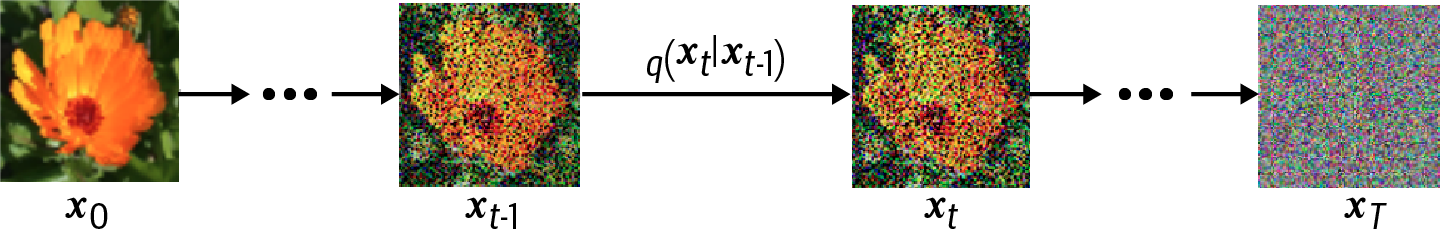
\includegraphics[width=0.95\textwidth]{figures/forward_diffusion_process}
	\end{center}
	\caption{The forward diffusion process}\label{fig:forward_diffusion_process}
\end{figure}


We can write this update process mathematically as follows (here, \( \epsilon_{t-1} \) is a standard Gaussian with zeor mean and unit variance):

\[
	\mathbf{x}_t = \sqrt{1 - \beta_t}  \mathbf{x}_{t-1} + \sqrt{\beta_t} \epsilon_{t-1}
	.\]

Note that we also scale the input image \( \mathbf{x}_{t-1}\), to ensure that the variance of the output image \( \mathbf{x}_t \) remains constant over time.
This way, if we normalize our original image \( \mathbf{x}_0 \) to have zeor mean and unit variance, the \( \mathbf{x}_t \) will approximate a standard Gaussian distribution for large enough \( T \), by induction, as follows.

If we assume that \( \mathbf{x}_{t-1} \) has zeor mean and unit variance then \( \sqrt{1 - \beta_t} \mathbf{x}_{t-1} \)  will have variance \( 1- \beta _t \) and \( \sqrt{\beta _t} \epsilon_{t-1}  \) will have variance \( \beta _t \), using the rule that \( \mathrm{Var}\left(aX\right) = a^2 \mathrm{Var}\left(X\right) \).
Adding these together, we obtain a new distribution \( \mathbf{x}_t \) with zero mean and variance \( 1- \beta _t + \beta _t =  1\), using the rule that \( \mathrm{Var}\left(X+Y\right) = \mathrm{Var}\left(X\right) \mathrm{Var}\left(Y\right)\) for independent \( X \) and \( Y \).
Therefore, if \( \mathbf{x}_0 \) is normalized to a zero mean and unit variance, then we guarantee that this is also true for  all \( \mathbf{x}_t \), including the final image \( \mathbf{x}_T \), which will approximate a standard Gaussian distribution.
This is exactly what we need, as we want to be alble to easily sample \( \mathbf{x}_T \) and then apply a reverse diffusion process through our trained neural network model.

In other words, our forward nosing process \( q \) can also be written as follows:

\[
	q(\mathbf{x}_t  \mid  \mathbf{x}_{t-1}) = \mathcal{N}(\mathbf{x}_t; \sqrt{1- \beta _t} \mathbf{x}_{t-1}, \beta _t \mathbf{I})
	.\]

\paragraph{The Reparmeaterization Trick}

It would also be useful to be able to jump straight from an image \( \mathbf{x}_0 \) to any noised version of the image \(  \mathbf{x}_t\) without having to go through \( t \) applications of \( q \).


If we define \( \alpha = 1 - \beta_t  \) and \( \overline{\alpha}_t  = \prod_{i=1}^{t} \alpha_i \), then we can write the following:

\begin{align*}
	\mathbf{x}_t & = \sqrt{\alpha_t} \mathbf{x}_{t-1} + \sqrt{1- \alpha_t} \epsilon_{t-1}                      \\
	             & = \sqrt{\alpha_t \alpha_{t-1}} \mathbf{x}_{t-2} + \sqrt{1- \alpha _t \alpha_{t-1}} \epsilon \\
	             & = \ldots                                                                                    \\
	             & = \sqrt{\overline{\alpha}_t}  \mathbf{x}_0 + \sqrt{1- \overline{\alpha }_t} \epsilon
	.\end{align*}


Note that the second line uses the fact that we can add two Gaussians to obtain a new Gaussian.
We therefore have have a way to jump from the original image \( \mathbf{x}_0 \) to nay step of the forward diffusion process \( \mathbf{x}_t \).
Moverover, we can define the diffusion schedule using the \( \overline{\alpha }_t \)values, instead of the original \( \beta _t \) values, with the interpretation that \( \overline{\alpha }_t \) is the variance due to the signal (the original image, \( \mathbf{x}_0 \)) and \( 1 - \overline{\alpha }_t \) is the variance due to the noise (\( \epsilon \)).

The forward diffusion process \( q \) can therefore also be written as follows:

\[
	q\left(\mathbf{x}_t  \mid  \mathbf{x}_0\right) = \mathcal{N}\left(\mathbf{x}_t; \sqrt{\overline{\alpha }_t } \mathbf{x}_0, \left(1 - \overline{\alpha }_t\right) \mathbf{I}\right)
	.\]

\paragraph{Diffusion Schedule}

Notice that we are also free to choose a different \( \beta_t \) at each timestep—they don’t all have be the same.
How the \( \beta_t \) (or \( \hat{\alpha}_t \) ) values change with \( t \) is called the diffusion schedule.

In the original paper~\cite{hoogeboom2021autoregressive}, the authors chose a linear diffusion schedule for \( \beta_t \) that is, \( \beta_t \) increases linearly with \( t \), from  \(  \beta_1 = 0.0001 \) to \( \beta_T = 0.02 \).
This ensures that in the early stages of the noising process we take smaller noising steps than in the later stages, when the image is already very noisy.


In a later paper it was found that a cosine diffusion schedule outperformed the linear schedule from the original paper~\cite{hoogeboom2021autoregressive}.
A cosine schedule defines the following values of \( \hat{\alpha}_t \):

\[
	\hat{\alpha}_t = \cos \left(\frac{\pi t}{2T}\right)
	.\]

The updated equation is therefore as follows (using the trigonometric identity \( \cos ^{2} \left(x\right) + \sin ^2 = 1  \))

\[
	\mathbf{x}_t = \cos \left(\frac{t}{T} \cdot \frac{\pi }{2}\right) \mathbf{x}_0 + \sin \left(\frac{t}{T} \cdot \frac{\pi}{2}\right) \epsilon
	.\]


This equation is a simplified version of the actual cosine diffusion schedule used in the paper.
The authors also add an offset term and scaling to prevent the noising steps from being too small at the beginning of the diffusion process.
We can code up the cosine and offset cosine diffusion schedules as shown below:

\begin{minted}{python}
def cosine_diffusion_schedule(diffusion_times):
    signal_rates = tf.cos(diffusion_times * math.pi / 2)
    noise_rates = tf.sin(diffusion_times * math.pi / 2)
    return noise_rates, signal_rates

def offset_cosine_diffusion_schedule(diffusion_times):
    min_signal_rate = 0.02
    max_signal_rate = 0.95
    start_angle = tf.acos(max_signal_rate)
    end_angle = tf.acos(min_signal_rate)
    diffusion_angles = start_angle + diffusion_times * (end_angle - start_angle)
    signal_rates = tf.cos(diffusion_angles)
    noise_rates = tf.sin(diffusion_angles)
\end{minted}

\paragraph{The Reverse Diffusion Process}

There are many similarities between the the reverse diffusion proceess and the decoder of a variational autoencoder.


\paragraph{Sampling from the Denoising Diffusion Model}

In order to sample images from trained model, we need to apply the reverse diffusion process, that is, we need to start with random noise adn use the model to gradually undo the noise, until we are left with recognizable picture of a flower.
However, we do not want to undo the noise all in one go in which predicting an image from pure random noise in one shot is clearly not going to work.
We would rather mimic the forward process and undo the predicted noise gradually over many small steps, to allow the model to adjust to its own predictions.

To achieve this, we can jump from \( x_t \) to \( x_{t-1} \) in two steps, first by using our model's noise prediction to calculate an estimate for the original image \( x_{0} \) and the by replying the predicted noise to this image, but only over \( t-1 \) timesteps, to produce \( x_{t-1} \)~\pautoref{fig:one_step_difussion_model}.

\begin{figure}
	\begin{center}
		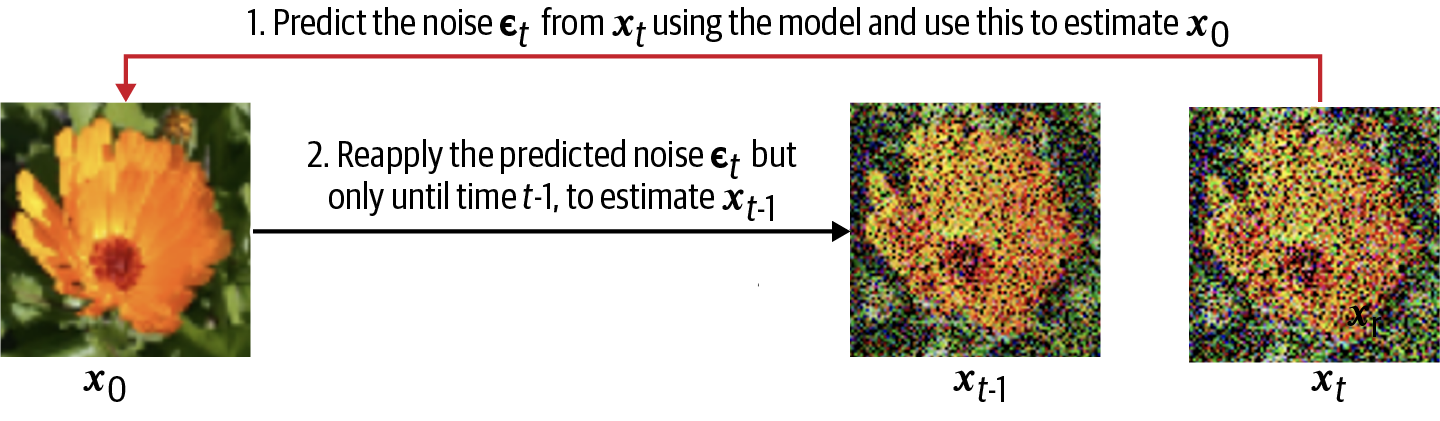
\includegraphics[width=0.95\textwidth]{figures/one_step_difussion_model}
	\end{center}
	\caption{One step of the sampling process for our diffusion model~\cite{foster2022generative}}\label{fig:one_step_difussion_model}
\end{figure}

If we repeat this process over a number of steps, we’ll eventually get back to an estimate for \( x_{0} \) that has been guided gradually over many small steps.
In fact, we are free to choose the number of steps we take, and crucially, it doesn’t have to be the same as the large number of steps in the training noising process (i.e., \num{1,000}).
It can be much smaller—in this example we choose \num{20}.

The following equation~\cite{song2022denoising} this process mathematicaly:

\[
	\mathbf{x}_{t-1} = \sqrt{\overline{\alpha}_{t-1}} \left(\frac{\mathbf{x}_t - \sqrt{1- \overline{\alpha }_t} \epsilon ^{(t)}_\theta\left(\mathbf{x}_t\right)  }{\sqrt{\overline{\alpha }_t} }\right) + \sqrt{1 - \overline{\alpha }_{t-1} - \sigma ^2_t } \cdot \epsilon ^{(t)}  _\theta \left(\mathbf{x}_t\right) + \sigma _t \epsilon_t
	.\]

Let's break this down.
The first term inside the brackets on the righthand side of the equation is the estimated image \( x_{0} \), calculated using the noise predicted by our network \( \epsilon ^{(t)} _\theta \).
We then scale this by the \( t-1 \) signal rate \( \sqrt{\overline{\alpha}_t - 1} \) and reapply the predicted noise, but this time scaled by the \( t - 1 \) noise rate \( \sqrt{1 - \overline{\alpha}_{t-1}  \sigma ^2 _t } \).
Additional Gaussian random noise \( \sigma _t \epsilon_t \) is also added, with the factors \( \sigma _t \) determining how random we want our generation process to be.

The special case \( \sigma _t = 0 \) for all \( t \) corresponds to a type of model known as a \gls{ddim}, introduced by \textcite{song2022denoising}.
With \gls{ddim}, the generation process is entirely deterministic, which is the same random noise input will always give the same output.
This is desirable as the we have a well-defined mapping between samples from the latent space and the generated output in pixel space.


\paragraph{Analysis of the Diffusion Model}

\begin{figure}
	\begin{center}
		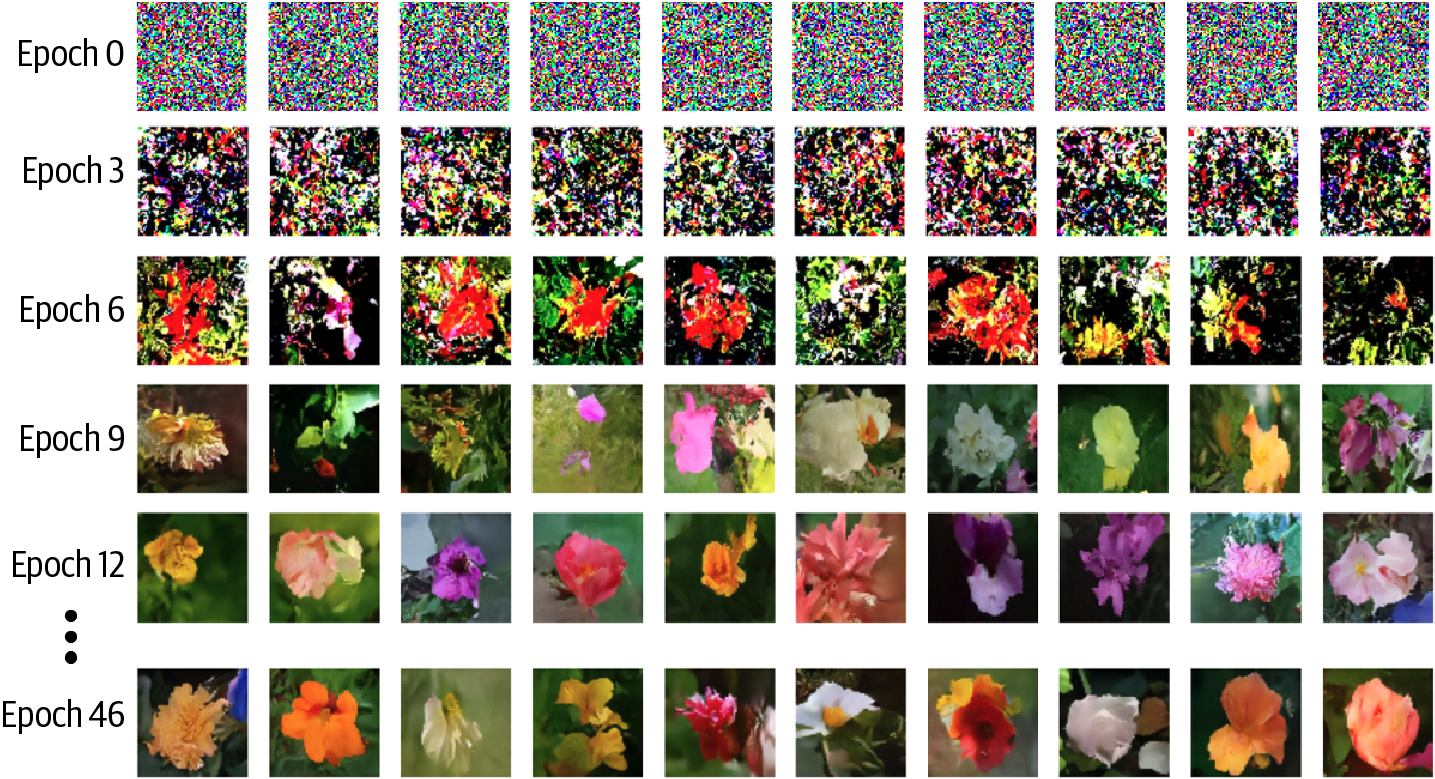
\includegraphics[width=0.95\textwidth]{figures/samples_from_diffussion_models}
	\end{center}
	\caption{Samples from the diffusion model at different epochs of the training process~\cite{foster2022generative}}\label{fig:samples_from_diffussion_models}
\end{figure}

We can see in~\autoref{fig:samples_from_diffussion_models} that the quality of the generations does indeed improve with the number of diffusion steps.
With one giant leap from the initial sampled noise, the model can only predict a hazy blob of color.
With more steps, the model is able to refine and sharpen its generations.
However, the time taken to generate the images scales linearly with the number of diffusion steps, so there is a trade-off.
There is minimal improvement between \num{20} and \num{100} diffusion steps, so we choose \num{20} as a reasonable compromise between quality and speed in this example~\cite{foster2022generative}.

The reverse diffusion process is parameterized by a U-Net that tries to predict the noise at each timestep, given the noised image and the noise rate at that step.
A U-Net consists of DownBlocks that increase the number of channels while reducing the size of the image and UpBlocks that decrease the number of channels while increasing the size.
The noise rate is encoded using sinusoidal embedding~\cite{foster2022generative}.

Sampling from the diffusion model is conducted over a series of steps.
The U-Net is used to predict the noise added to a given noised image, which is then used to calculate an estimate for the original image.
The predicted noise is then reapplied using a smaller noise rate.
This process is repeated over a series of steps (which may be significantly smaller than the number of steps used during training), starting from a random point sampled from a standard Gaussian noise distribution, to obtain the final generation~\cite{foster2022generative}.

We saw how increasing the number of diffusion steps in the reverse process improves the image generation quality, at the expense of speed.
We also performed latent space arithmetic in order to interpolate between two images~\cite{foster2022generative}.

\section{Transformers}

A recurrent layer tries to build up a generic hidden state that captures an overall representation of the input at each timestep.
A weakness of this approach is that many of the words that have already been incorporated into the hidden vector will not be directly relevant to the immediate task at hand (e.g., predicting the next word), as we have just seen.
Attention heads do not suffer from this problem, because they can pick and choose how to combine information from nearby words, depending on the context.


\begin{figure}
	\begin{center}
		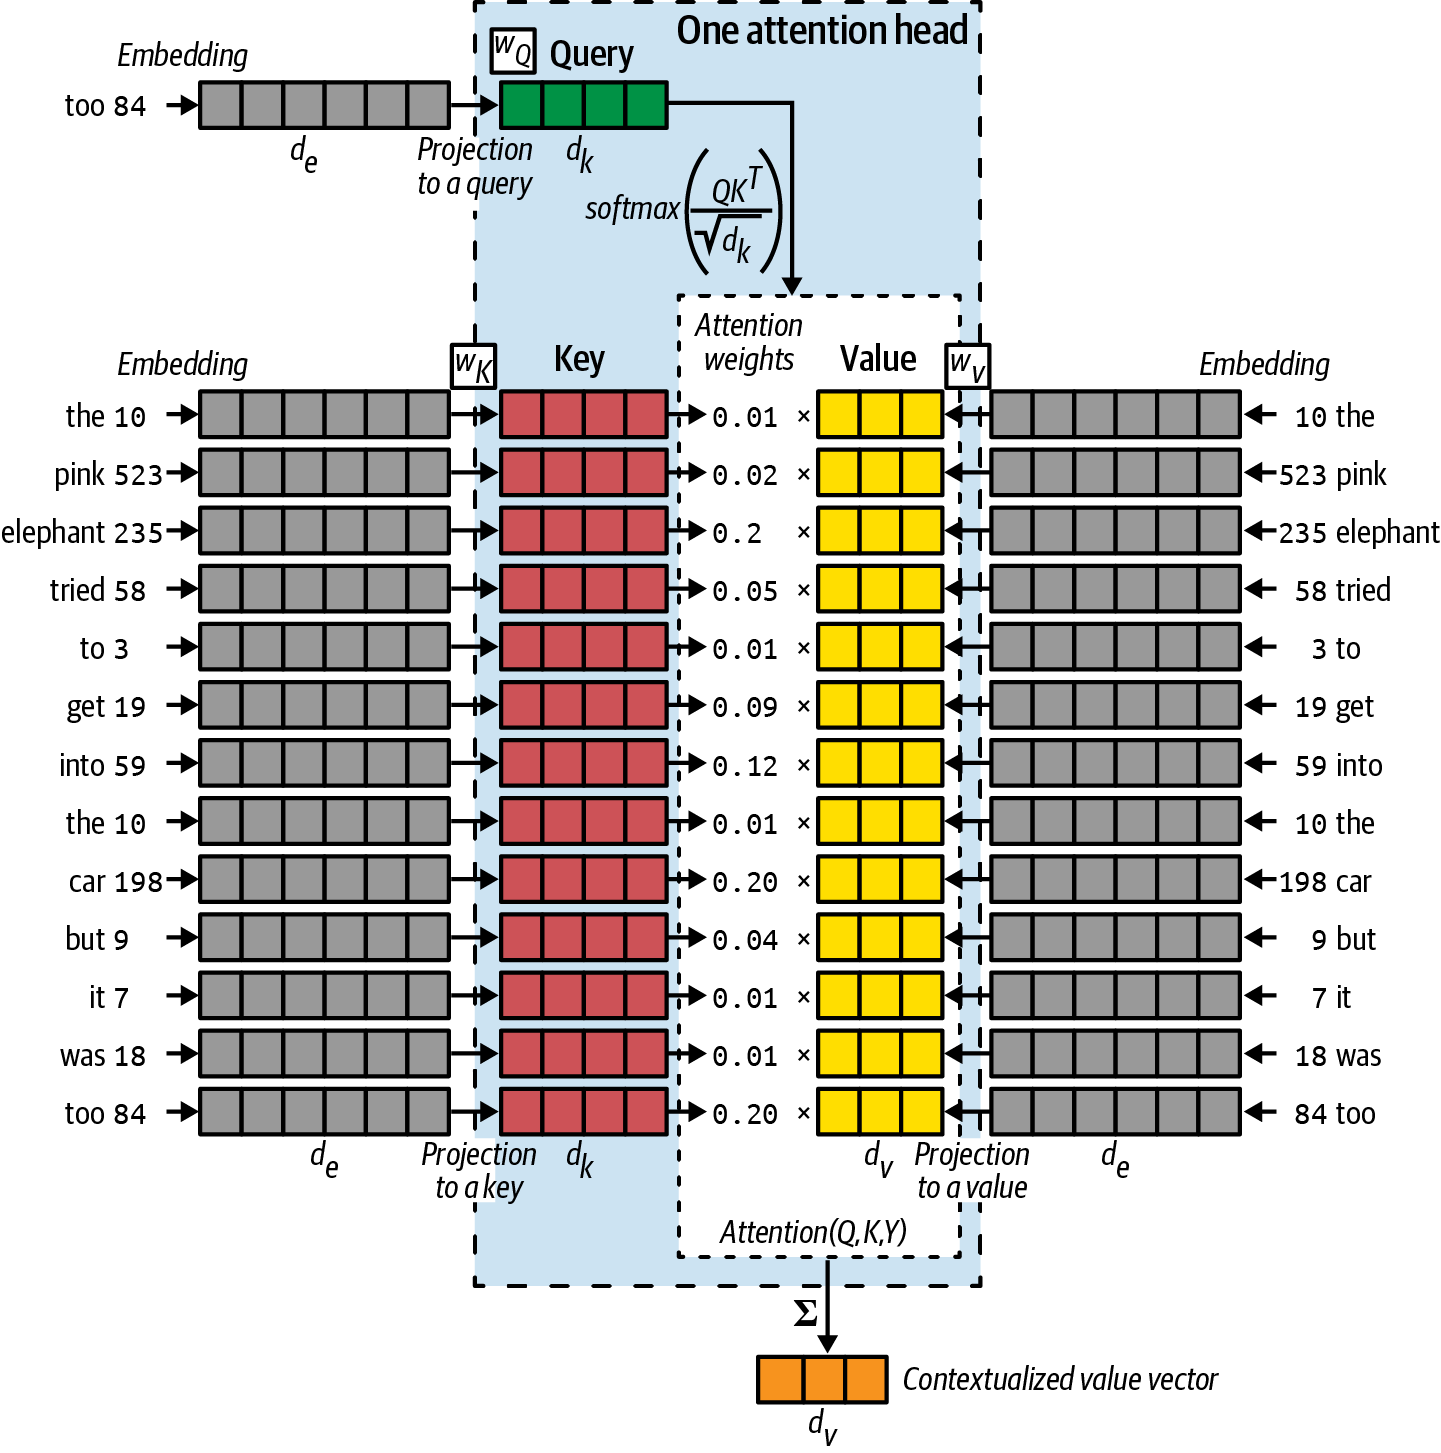
\includegraphics[width=0.95\textwidth]{figures/attention_1}
	\end{center}
	\caption{The mechanics of an attention head~\cite{foster2022generative}}\label{fig:attention_1}
\end{figure}

The query (\(Q\)) can be thought of as a representation of the current task at hand (e.g., ``What word follows too?'').
In this example, it is derived from the embedding of the word too, by passing it through a weights matrix \( W_Q \) to change the dimensionality of the vector from \( d_e \) to \( d_k \)~\pautoref{fig:attention_1}.

The key vectors (\( K \)) are representations of each word in the sentence—you can think of these as descriptions of the kinds of prediction tasks that each word can help with.
They are derived in a similar fashion to the query, by passing each embedding through a weights matrix \( W_K \) to change the dimensionality of each vector from \( d_e \) to \( d_k \).
Notice that the keys and the query are the same length (\( d_k \)).


Inside the attention head, each key is compared to the query using a dot product between each pair of vectors (\( QK^{T} \)).
This is why the keys and the query have to be the same length.
The higher this number is for a particular key/query pair, the more the key resonates with the query, so it is allowed to make more of a contribution to the output of the attention head.
The resulting vector is scaled by  \( \sqrt{d_k} \) to keep the variance of the vector sum stable (approximately equal to 1), and a softmax is applied to ensure the contributions sum to 1.
This is a vector of \emph{attention weights}.

The value vectors (\( V \)) are also representations of the words in the sentence—you can think of these as the unweighted contributions of each word.
They are derived by passing each embedding through a weights matrix \( W_V \) to change the dimensionality of each vector from  \( d_e \)to \( d_v \).
Notice that the value vectors do not necessarily have to have the same length as the keys and query (but often do, for simplicity).

The value vectors are multiplied by the attention weights to give the attention for a given \( Q \), \( K \), and \( V \), as shown in~\autoref{eq:attention}.

\begin{equation}
	\mathrm{Attention}(Q, K, V) = \mathrm{softmax}\left(\frac{QK^{T}}{\sqrt{d_k}}\right)V
	\label{eq:attention}
\end{equation}

\paragraph{Multi-Head Attention}

The concatenated outputs are passed through one final weights matrix \(W_O\) to project the vector into the desired output dimension, which in our case is the same as the input dimension of the query (\( d_e \)), so that the layers can be stacked sequentially on top of each other~\pautoref{fig:multi_head}.

\begin{figure}
	\begin{center}
		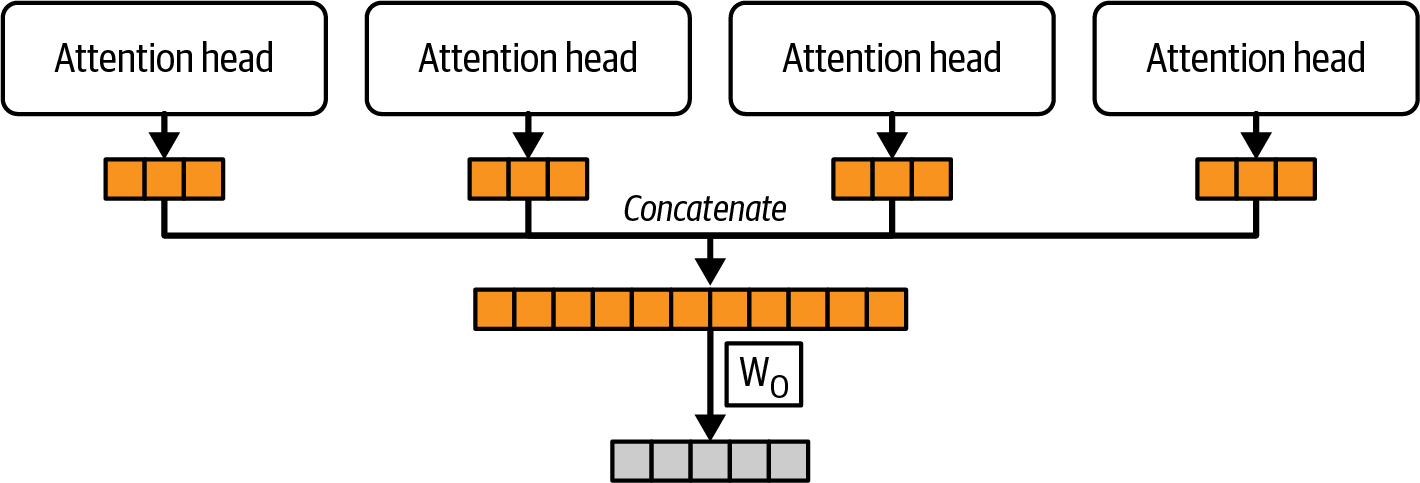
\includegraphics[width=0.95\textwidth]{figures/multi_head}
	\end{center}
	\caption{The Multi-Head Attention}\label{fig:multi_head}
\end{figure}

\paragraph{Causal Masking}

Causal masking is only required in decoder Transformers such as GPT, where the task is to sequentially generate tokens given previous tokens.
Masking out future tokens during training is therefore essential~\pautoref{fig:causal_mask}.

Other flavors of Transformer (e.g., encoder Transformers) do not need causal masking, because they are not trained to predict the next token~\cite{vaswani2017attention}.
For example Google’s \gls{bert} predicts masked words within a given sentence, so it can use context from both before and after the word in question.
We will explore the different types of Transformers in more detail at the end of the chapter.

\begin{figure}
	\begin{center}
		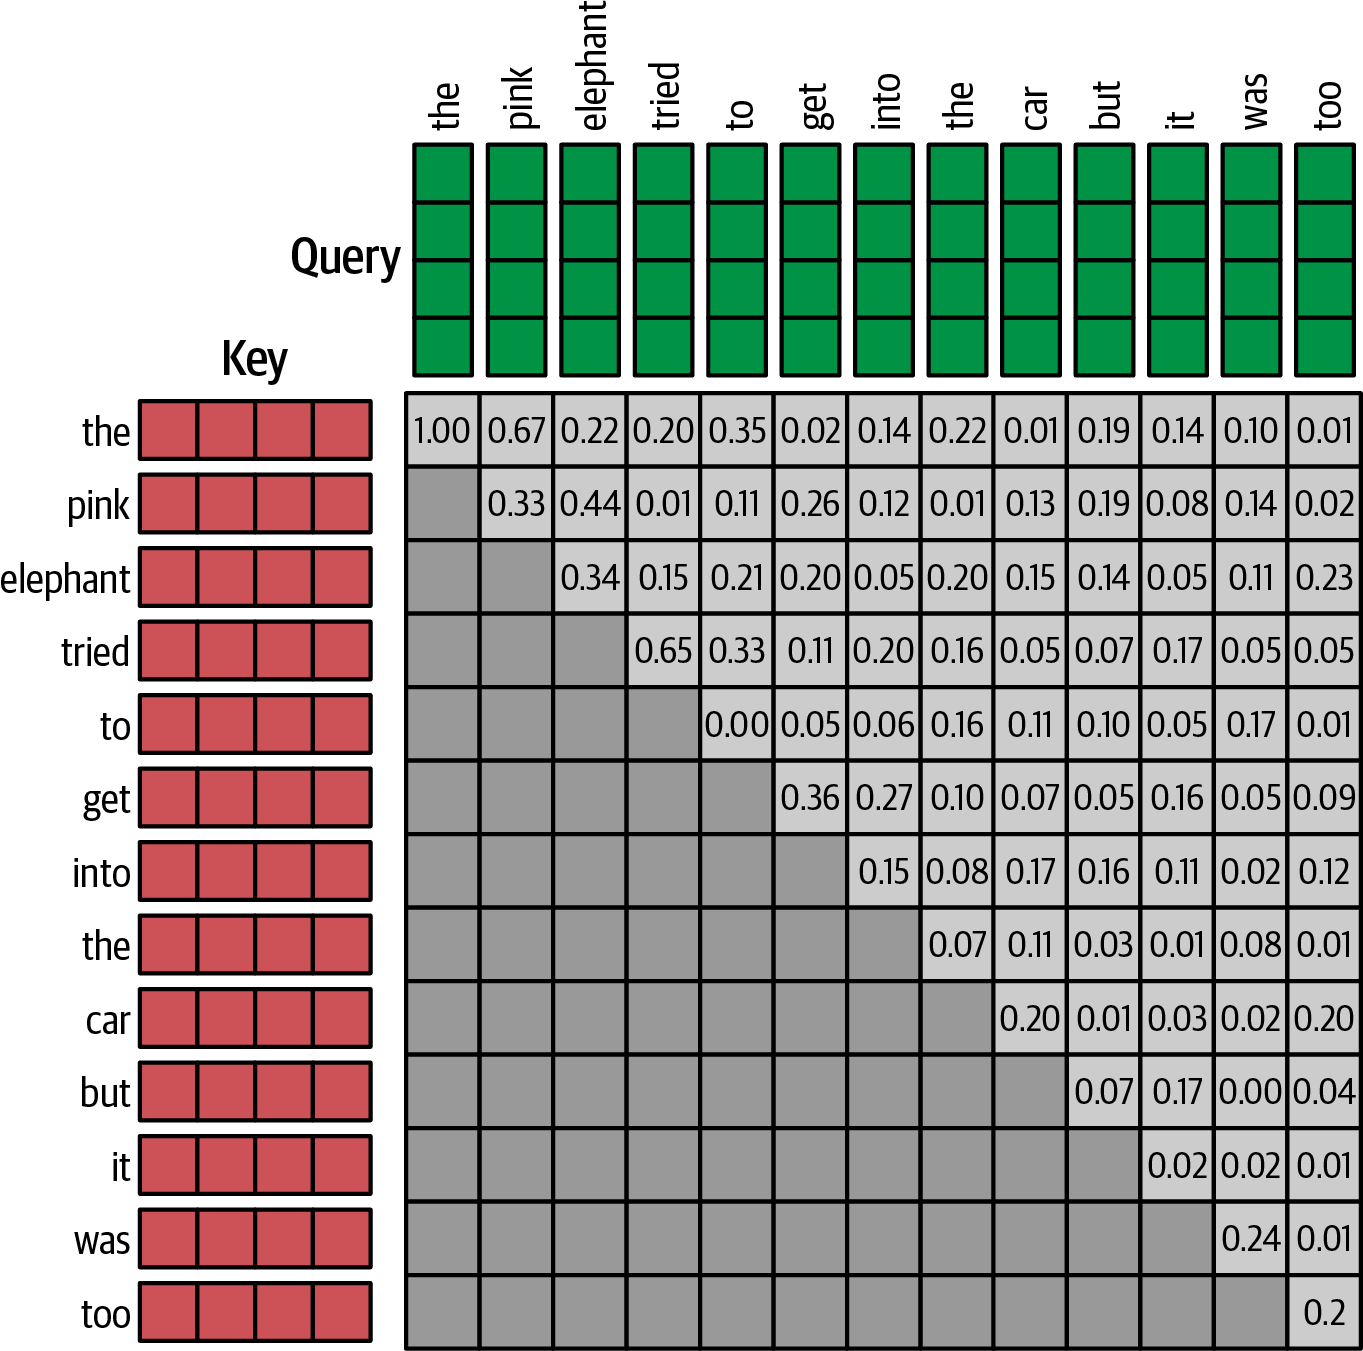
\includegraphics[width=0.95\textwidth]{figures/causal_mask}
	\end{center}
	\caption{Matrix calculation of the attention scores for a batch of input queries, using a causal attention mask to hide keys that are not available to the query (because they come later in the sentence)}\label{fig:causal_mask}
\end{figure}

This concludes our explanation of the multihead attention mechanism that is present in all Transformers.
It is remarkable that the learnable parameters of such an influential layer consist of nothing more than three densely connected weights matrices for each attention head ( \( W_Q, W_K, W_V \)) and one further weights matrix to reshape the output (\( W_O \)).
There are no convolutions or recurrent mechanisms at all in a multihead attention layer!

\paragraph{The Transformer Block~\pautoref{fig:transformer_block}}

\begin{figure}
	\begin{center}
		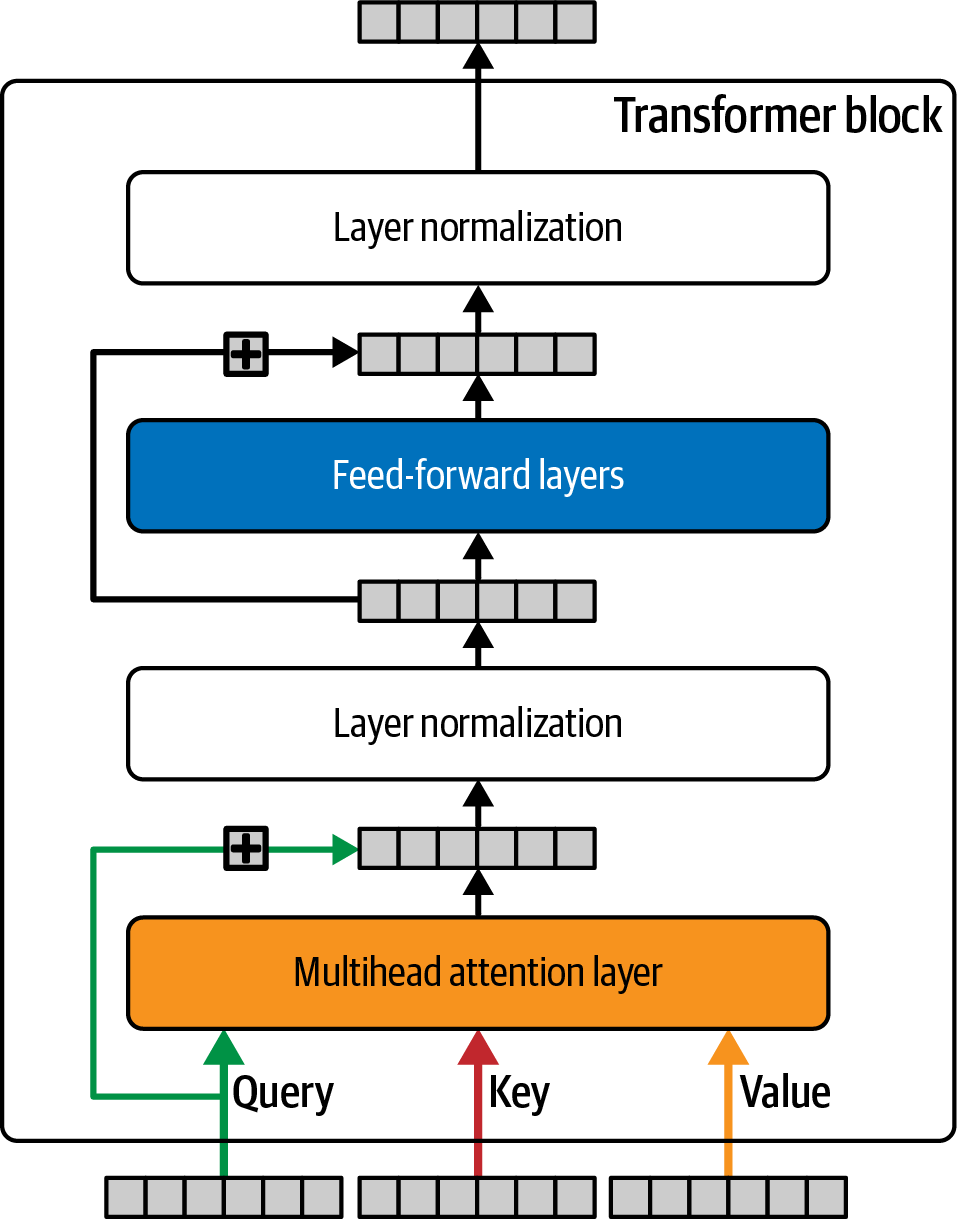
\includegraphics[width=0.95\textwidth]{figures/transformer_block}
	\end{center}
	\caption{A Transformer Block~\cite{foster2022generative}}\label{fig:transformer_block}
\end{figure}

In contrast, layer normalization in a Transformer block normalizes each position of each sequence in the batch by calculating the normalizing statistics across the channels.
It is the complete opposite of batch normalization, in terms of how the normalization statistics are calculated.
A diagram showing the difference between batch normalization and layer normalization is shown in~\autoref{fig:layer_norm}.

Layer normalization was used in the original GPT paper and is commonly used for text-based tasks to avoid creating normalization dependencies across sequences in the batch~\autoref{fig:layer_norm}.
However, recent work such as \textcite{shen2020powernorm} challenges this assumption, showing that with some tweaks a form of batch normalization can still be used within Transformers, outperforming more traditional layer normalization.

\begin{figure}
	\begin{center}
		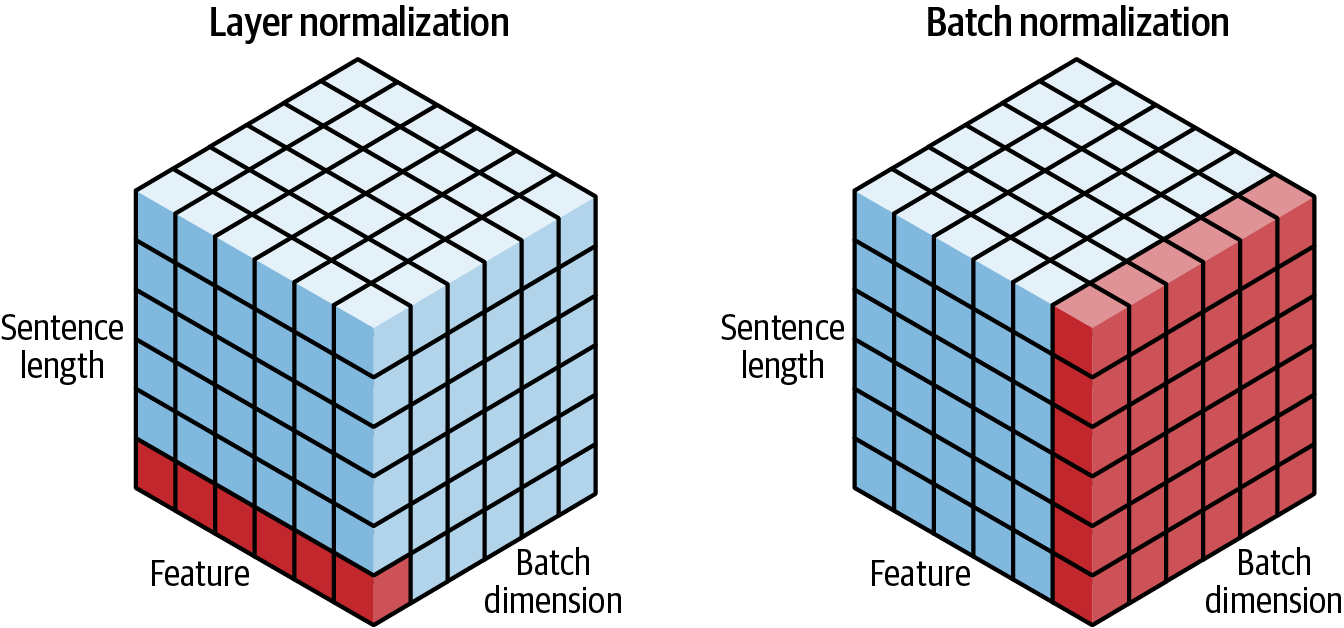
\includegraphics[width=0.95\textwidth]{figures/layer_norm}
	\end{center}
	\caption{Layer normalization versus batch normalization—the normalization statistics are calculated across the blue cells~\cite{shen2020powernorm}}\label{fig:layer_norm}
\end{figure}

\paragraph{Positional Embeddings}

To construct the joint token–position encoding, the token embedding is added to the positional embedding, as shown in~\autoref{fig:positional_embedding}.
This way, the meaning and position of each word in the sequence are captured in a single vector.

\begin{figure}
	\begin{center}
		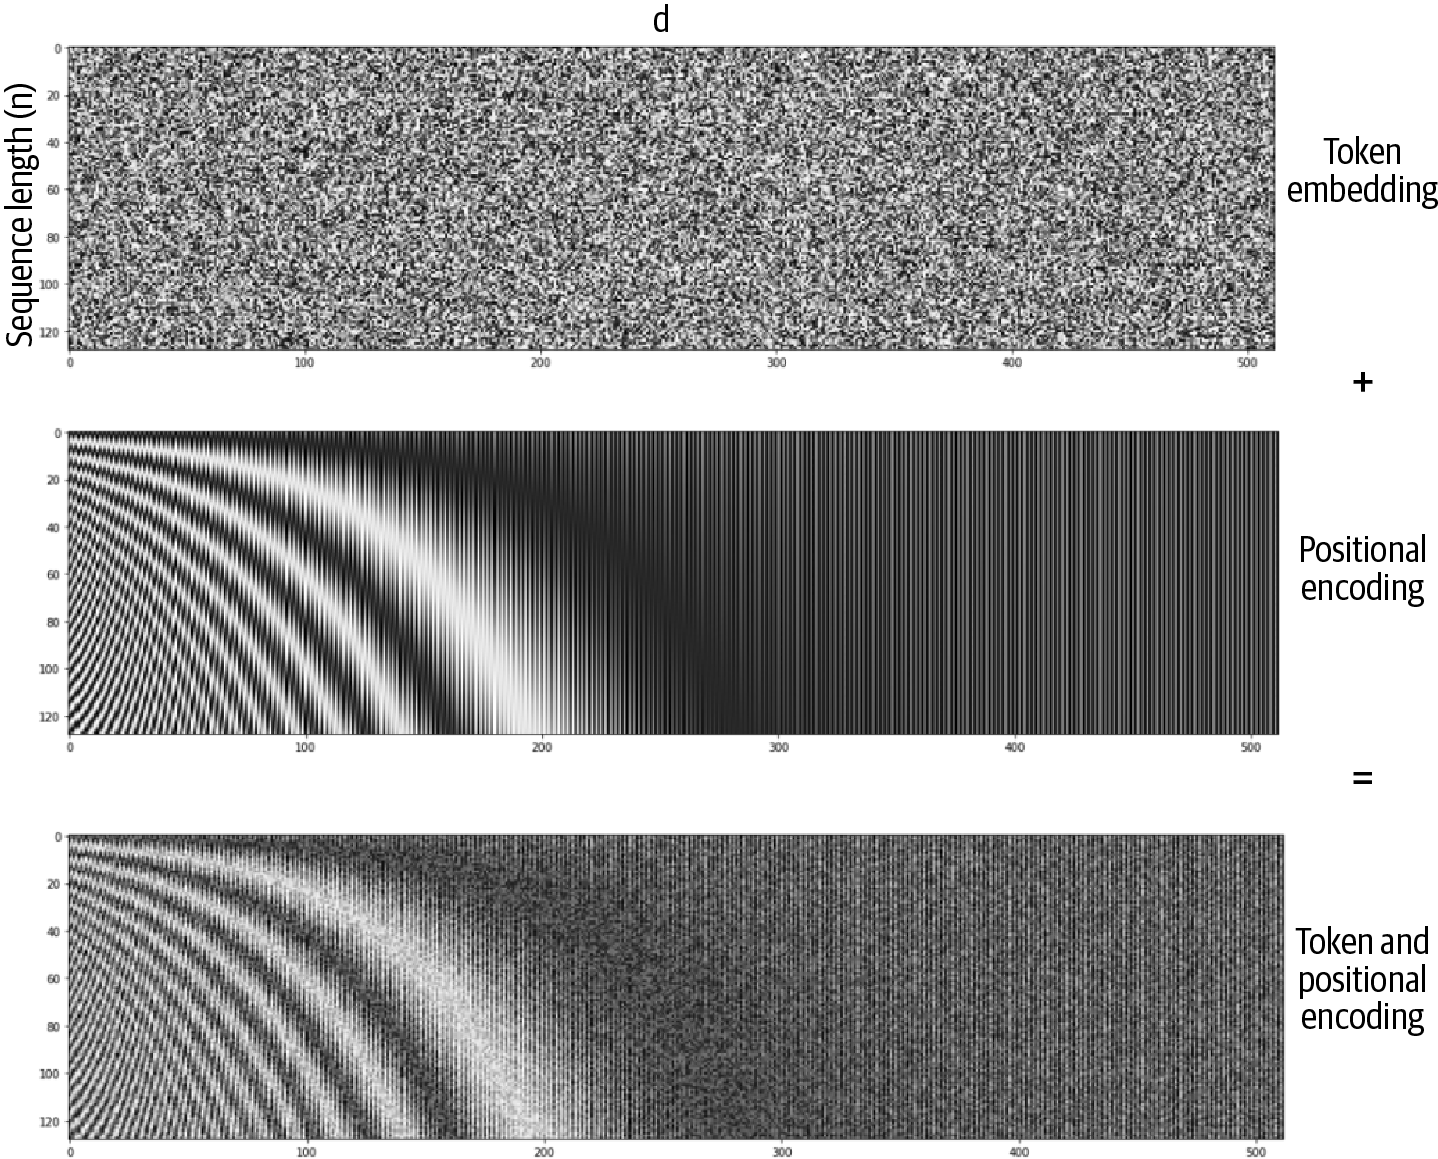
\includegraphics[width=0.9\textwidth]{figures/positional_embedding}
	\end{center}
	\caption{The token embeddings are added to the positional embeddings to give the token position encoding~\autoref{fig:positional_embedding}}\label{fig:positional_embedding}
\end{figure}

\paragraph{Summary}

Attention heads can be grouped together to form what is known as a multihead attention layer.
These are then wrapped up inside a Transformer block, which includes layer normalization and skip connections around the attention layer.
Transformer blocks can be stacked to create very deep neural networks.

Causal masking is used to ensure that \gls{gpt} cannot leak information from downstream tokens into the current prediction.
Also, a technique known as positional encoding is used to ensure that the ordering of the input sequence is not lost, but instead is baked into the input alongside the traditional word embedding.

When analyzing the output from \gls{gpt}, we saw it was possible not only to generate new text passages, but also to interrogate the attention layer of the network to understand where in the sentence it is looking to gather information to improve its prediction.
GPT can access information at a distance without loss of signal, because the attention scores are calculated in parallel and do not rely on a hidden state that is carried through the network sequentially, as is the case with recurrent neural networks.

We saw how there are three families of Transformers (encoder, decoder, and encoder-decoder) and the different tasks that can be accomplished with each.

\paragraph{The Illustrated Transformer~\cite{alammar2018illustrated}}

\begin{figure}
	\begin{center}
		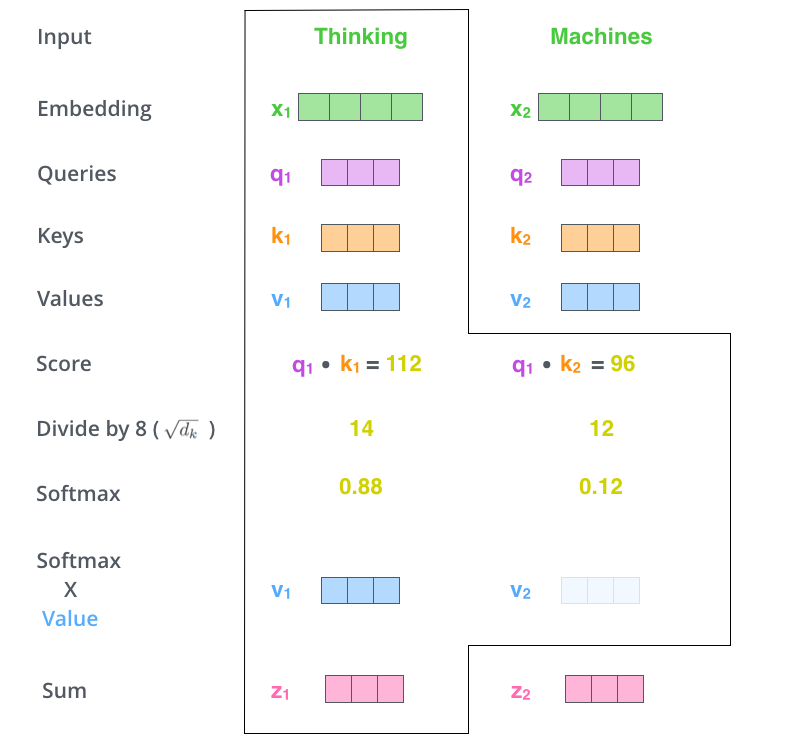
\includegraphics[width=0.9\textwidth]{figures/self-attention-output}
	\end{center}
	\caption{Self-attention Output}\label{fig:self-attention-output}
\end{figure}

Matrix calculation of self-attention is shown in~\autoref{fig:self-attention-matrix-calculation}.

\begin{figure}
	\begin{center}
		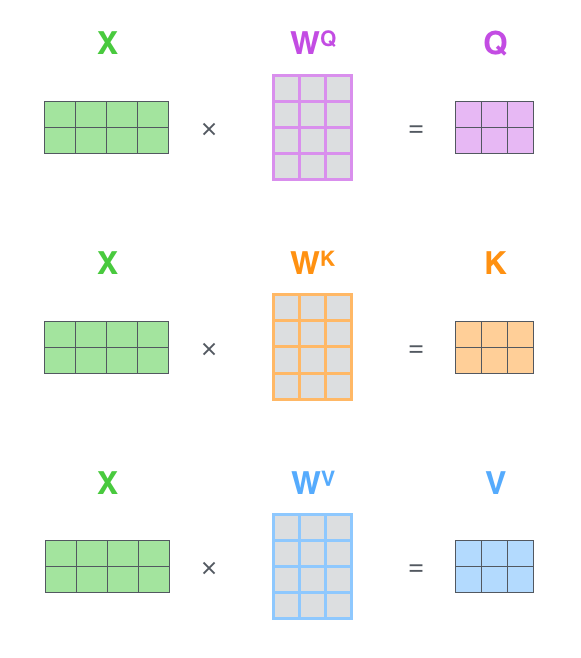
\includegraphics[width=0.9\textwidth]{figures/self-attention-matrix-calculation}
	\end{center}
	\caption{Self-attention Matrix Calculation}\label{fig:self-attention-matrix-calculation}
\end{figure}

Finally, since we’re dealing with matrices, we can condense steps two through six in one formula to calculate the outputs of the self-attention layer.

\begin{figure}
	\begin{center}
		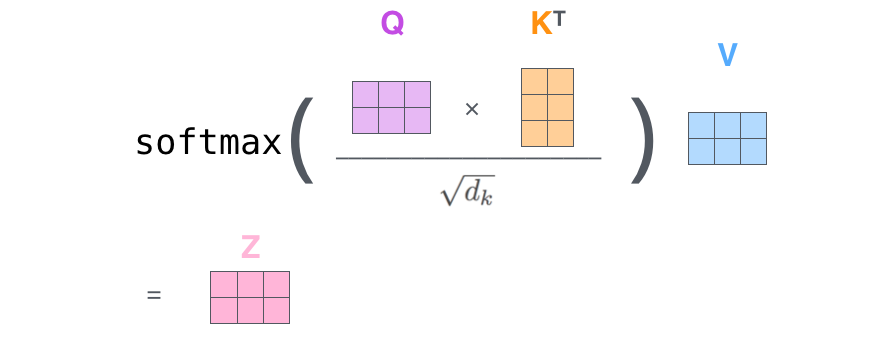
\includegraphics[width=0.9\textwidth]{figures/self-attention-matrix-calculation-2}
	\end{center}
	\caption{Self-attention Matrix Calculation}\label{fig:self-attention-matrix-calculation-2}
\end{figure}

Let me try to put them all in one visual so we can look at them in one place~\pautoref{fig:self-attention-matrix-calculation-2}.

\begin{figure}
	\begin{center}
		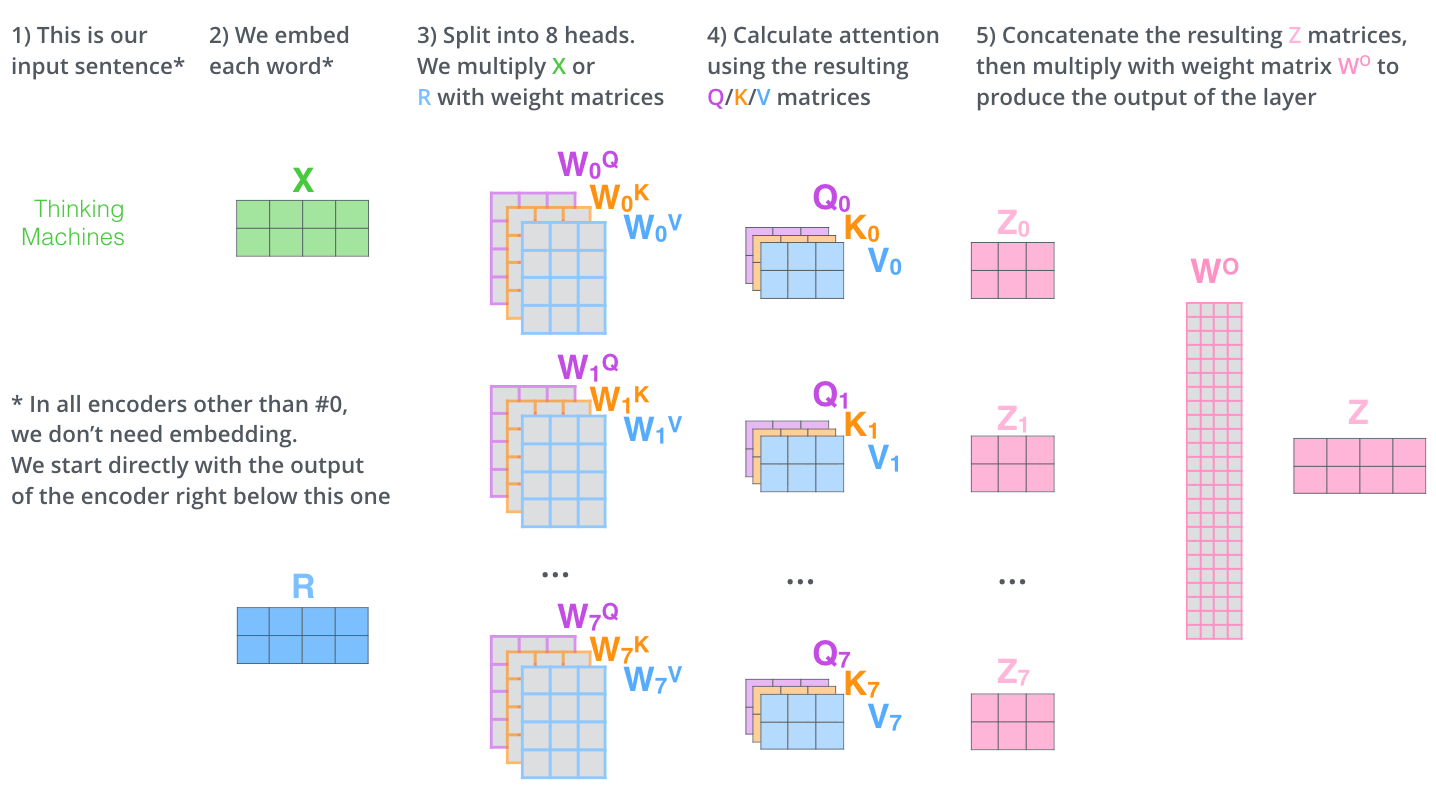
\includegraphics[width=0.9\textwidth]{figures/transformer_multi-headed_self-attention-recap}
	\end{center}
	\caption{Transformer Multi-headed Self-attention Recap}\label{fig:transformer_multi-headed_self-attention-recap}
\end{figure}

\section{Advanced \glspl{gan}}

The \href{https://github.com/hindupuravinash/the-gan-zoo}{\gls{gan} Zoo GitHub repository} is a great resource for exploring the different types of \glspl{gan} that have been proposed over the years.

\paragraph{\gls{progan}~\cite{Karras2018Feb}}

\gls{progan} is a technique developed by NVIDIA Labs in 2017 to improve both the speed and stability of \gls{gan} training.
Instead of immediately training a \gls{gan} on fullresolution images, the \gls{progan} paper suggests first training the generator and discriminator on low-resolution images of, say, \( 4 \times  4 \) pixels and then incrementally adding layers throughout the training process to increase the resolution.

In a normal \gls{gan}, the generator always outputs full-resolution images, even in the early stages of training.
It is reasonable to think that this strategy might not be optimal—the generator might be slow to learn high-level structures in the early stages of training, because it is immediately operating over complex, high-resolution images.
Wouldn’t it be better to first train a lightweight \gls{gan} to output accurate low-resolution images and then see if we can build on this to gradually increase the resolution?

This simple idea leads us to progressive training, one of the key contributions of the \gls{progan} paper.
The \gls{progan} is trained in stages, starting with a training set that has been condensed down to \( 4 \times   4 \) pixel images using interpolation, as shown in~\autoref{fig:progan}.

\begin{figure}
	\begin{center}
		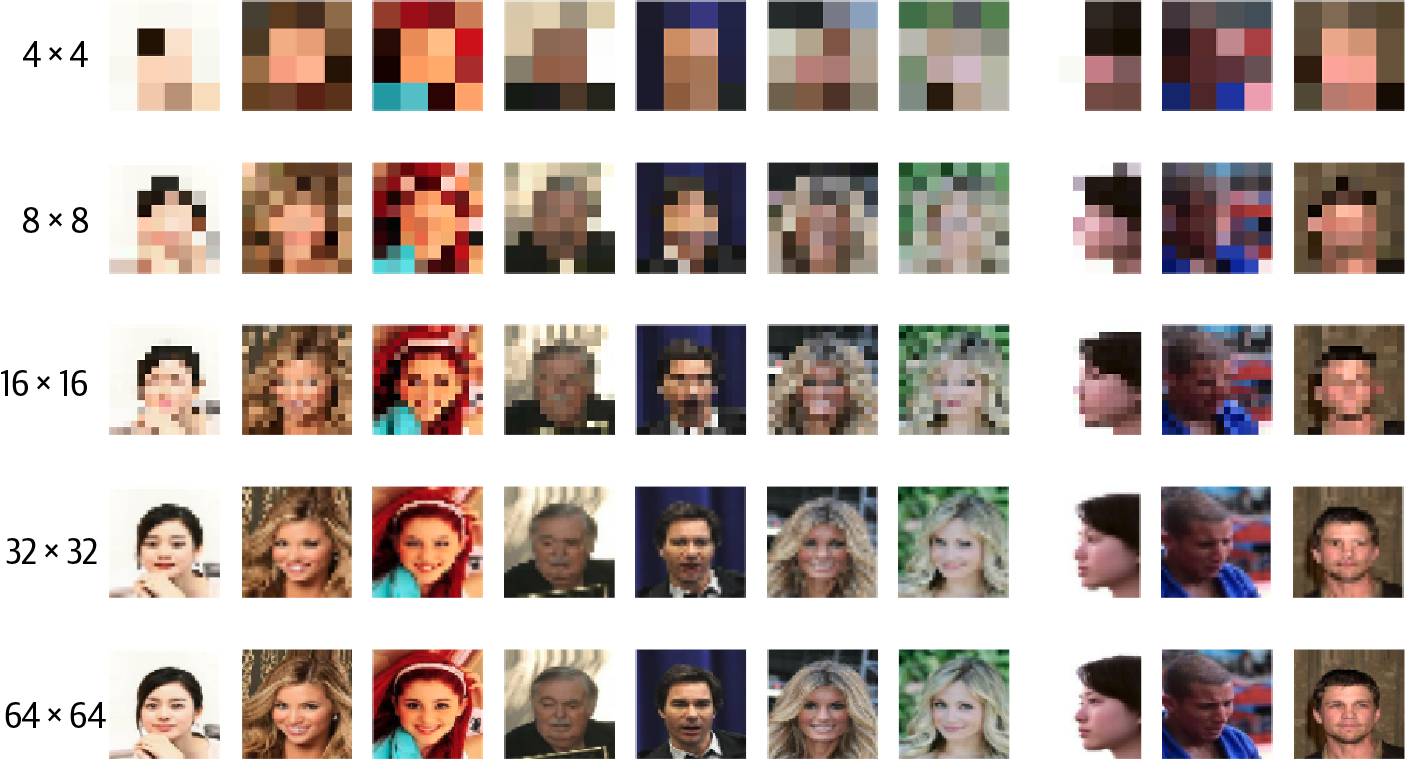
\includegraphics[width=0.95\textwidth]{figures/progan}
	\end{center}
	\caption{Images in the dataset can be compressed to lower resolution using interpolation}\label{fig:progan}
\end{figure}

Features:

\begin{itemize}
	\item Progressive training
	\item Minibatch standard deviation
	\item Equalized learning rate
	\item Pixelwise feature vector normalization
	\item Scaled images and pixel values
\end{itemize}

\paragraph{\gls{stylegan}~\cite{karras2018tyle}}

\gls{stylegan} is a \gls{gan} architecture from 2018 that builds on the earlier ideas in the \gls{progan} paper.
In fact, the discriminator is identical; only the generator is changed~\pautoref{fig:stylegan}.

\begin{figure}
	\begin{center}
		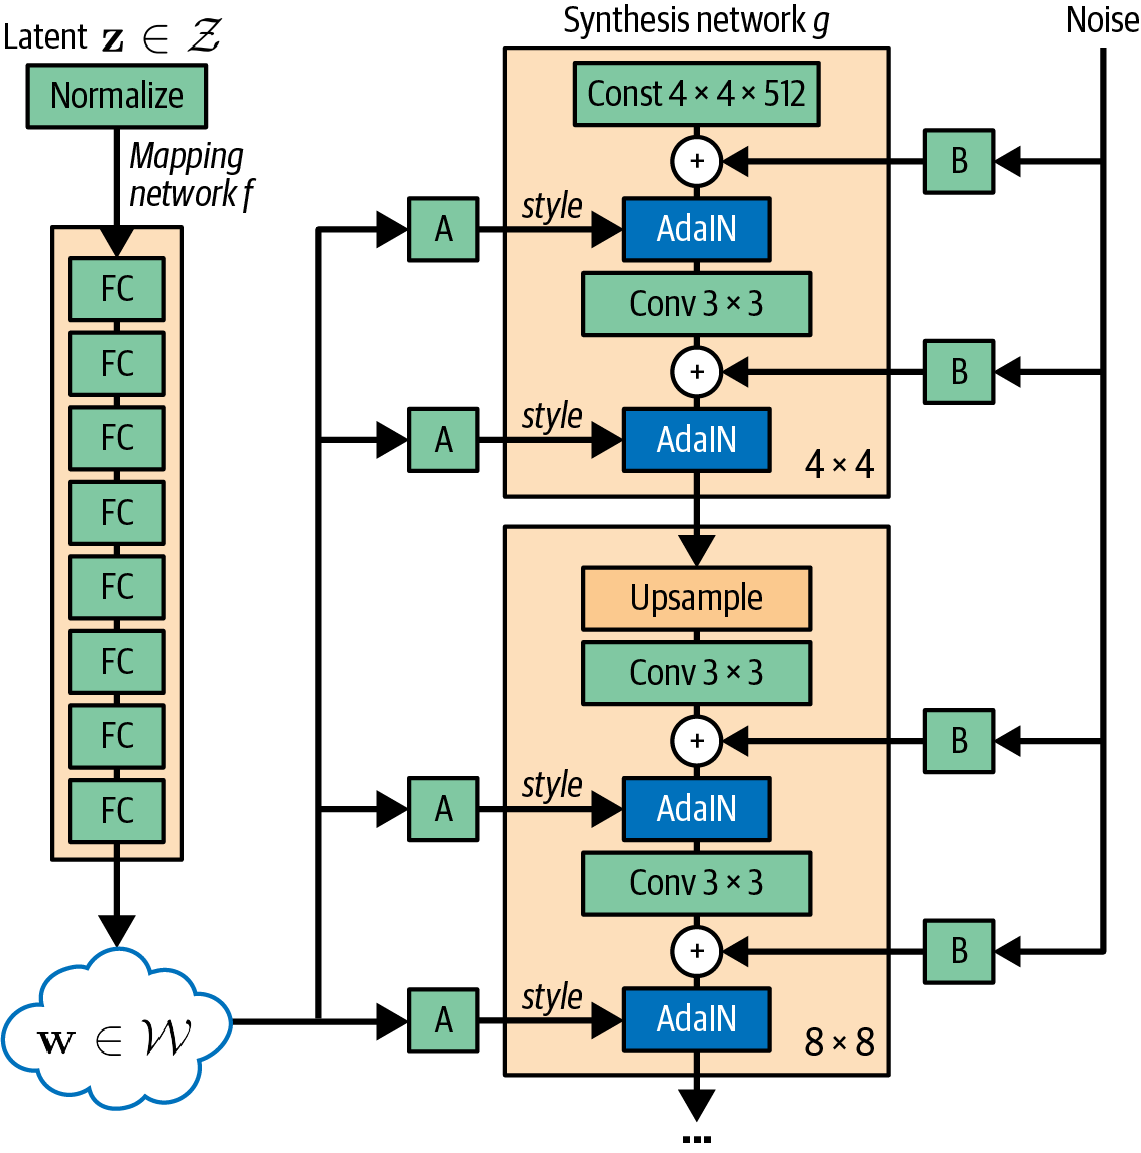
\includegraphics[width=0.9\textwidth]{figures/stylegan.png}
	\end{center}
	\caption{The \gls{stylegan} Generator Architecture}\label{fig:stylegan}
\end{figure}

Features:

\begin{itemize}
	\item The Mapping Network
	\item The Adaptive Instance Normalization Layer
	\item The Style Mixing Regularization
	\item Stochastic Variation
\end{itemize}

\paragraph{\gls{stylegan}2}

\begin{itemize}
	\item Weight Modulation and Demodulation
	\item Path Length Regularization
	\item No Progressive Growing
\end{itemize}

\paragraph{Summary}

We started by exploring the concept of progressive training that was pioneered in the 2017 \gls{progan} paper~\cite{Karras2018Feb}.
Several key changes were introduced in the 2018 \gls{stylegan} paper that gave greater control over the image output, such as the mapping network for creating a specific style vector and synthesis network that allowed the style to be injected at different resolutions.
Finally, \gls{stylegan}2 replaced the adaptive instance normalization of \gls{stylegan} with weight modulation and demodulation steps, alongside additional enhancements such as path regularization.
The paper also showed how the desirable property of gradual resolution refinement could be retained without having to the train the network progressively.

We also saw how the concept of attention could be built into a \gls{gan}, with the introduction of \gls{sagan} in 2018~\cite{zhang2019selfattention}.
This allows the network to capture long-range dependencies, such as similar background colors over opposite sides of an image, without relying on deep convolutional maps to spread the information over the spatial dimensions of the image.
BigGAN was an extension of this idea that made several key changes and trained a larger network to improve the image quality further~\cite{brock2019large}.

In the VQ-GAN paper, the authors show how several different types of generative models can be combined to great effect.
Building on the original VQ-VAE paper that introduced the concept of a VAE with a discrete latent space, VQ-GAN additionally includes a discriminator that encourages the VAE to generate less blurry images through an additional adversarial loss term.
An autoregressive Transformer is used to construct a novel sequence of code tokens that can be decoded by the VAE decoder to produce novel images.
The ViT VQ-GAN paper extends this idea even further, by replacing the convolutional encoder and decoder of VQ-GAN with Transformers.


